\documentclass[times, utf8, seminar]{fer}
\usepackage{booktabs}
%math packages
\usepackage{authblk}
\usepackage{mathtools}
\usepackage{amsmath}
\usepackage[binary-units=true]{siunitx}
%table of images
\usepackage{graphicx}
\usepackage{longtable}
\usepackage{adjustbox}

%%floor symbol
\DeclarePairedDelimiter\floor{\lfloor}{\rfloor}

%%SI unit notation
\makeatletter
\providecommand\add@text{}
\newcommand\tagaddtext[1]{%
  \gdef\add@text{#1\gdef\add@text{}}}% 
\renewcommand\tagform@[1]{%
  \maketag@@@{\llap{\add@text\quad}(\ignorespaces#1\unskip\@@italiccorr)}%
}
\makeatother


\begin{document}

% TODO: Navedite naslov rada.
\title{Uporaba steganografije u revezibilnoj deidentifikaciji}

% TODO: Navedite vaše ime i prezime.
\author{	Katarina Matić,
	Hrvoje Backović,
	Marin Oršić,\\
	Dino Rakipović,
	Ivan Relić,
	Filip Reškov	}

% TODO: Navedite ime i prezime mentora.

\voditelj{Slobodan Ribarić}

\maketitle

\tableofcontents

\chapter{Projektni zadatak}
\section{Opis projektnog zadatka}
\section{Pregled i opis srodnih rješenja}

\paragraph{}
Steganografija se koristila od davnina i stoga su dosad razvijeni brojni postupci koji efektivno skrivaju i prenose tajne poruke putem raznih medija kao što su tekst, zvučni signali ili slike. Za potrebe ovog projekta, koncentriramo se na steganografske postupke koji se odnose na skrivanje podataka unutar slika jer svi oni mogu poslužiti u različitim situacijama za rješavanje problema koji se u ovom projektu rješava. Najprije ćemo nabrojati svojstva koja steganografski postupak treba zadovoljavati da bi bio praktično upotrebljiv. Ta svojstva ćemo koristiti kao mjeru po kojoj ćemo uspoređivati različite postupke. Nakon toga ćemo navesti i opisati nekoliko poznatih postupaka te ćemo ih usporediti sa našim algoritmom po svojstvima koje smo naveli.
\paragraph{}
Općenito, steganografske postupke nad slikama možemo klasificirati u dvije domene:
\textbf{transformacijska domena} (tehnika frekvencijske domene) i \textbf{slikovna domena} (tehnika prostorne domene). Transformacijska domena primjenjuje transformacije slike kako bi ubacio tajne podatke u sliku, dok slikovna domena koristi modificiranje bitova boje/intenziteta piksela i manipulaciju šuma u originalnoj slici. LSB algoritam koji se koristi u ovom projektu spada u slikovnu domenu steganografskih tehnika.Veliki broj istraživača su predložili brojne tehnike za ove domene koje čitatelj može dodatno proučiti u navedenoj literaturi [LITERATURA], a mi ćemo opisati samo neke najvažnije.
\paragraph{}
Za početak navodimo svojstva koja su važna za svaki steganografski postupak i po kojima ih uspoređujemo:
\begin{description}

\item[kapacitet] Vrlo je važno definirati kapacitet postupka, odnosno koliko podataka može najviše sakriti unutar medija (slike) bez da uzrokuje vidljive promjene na slici koje će potencijalnom napadaču dati do znanja da se u slici krije neka skrivena poruka.
\item[transparentnost] Nakon procesa skrivanja poruke, originalna slika će se u određenoj mjeri promijeniti. Mjera u kojoj stego-slika odudara od originalne se naziva transparentnost i poželjno je da ta razlika bude što manja kako bi bila manja šansa za otkrivanje kodirane poruke.
\item[robusnost]  Nakon što smo kodirali poruku unutar slike, poželjno je da ta poruka ostane nepromijenjena čak i ako slika bude podvrgnuta raznim transformacijama kao što je rezanje dijelova slike, skaliranje, filtriranje, dodavanje šuma i sl. Robusnost je svojstvo koje nam to opisuje.
\item[otpornost na promjene poruke] Za dobar steganografski postupak trebalo bi biti teško promijeniti tajnu poruku, jednom kada je ona kodirana u sliku. Ako je ta otpornost mala, moguće je da napadač otkrije poruku, promijeni njen sadržaj i proslijedi dalje do odredišta i time uzrokuje štetu.
\item[računska složenost] Često je poželjno da postupak skrivanja poruke unutar slike i njenu rekonstrukciju iz slike bude što je moguće brži, tako da omogući primjene u npr. aplikacijama koje rade u stvarnom vremenu. Stoga često uspoređujemo postupke po njihovoj računskoj složenosti
\end{description}
\paragraph{}
Kod prenošenja slika, često se provodi kompresija slike prije slanja. Ovaj koncept je jako bitan jer utječe na dobar odabir steganografskog postupka. Postoje brojni algoritmi za kompresiju slika, a klasificiramo ih u dvije skupine: \textit{lossy} i \textit{lossless}.
\paragraph{}
\textit{Lossy} kompresija reducira količinu informacije koju je potrebno prenijeti tako da trajno gubi dio informacija sa slike, najčešće redundantne informacije. Miču se oni detalji koje ljudsko oko ne može razlikovati, što rezultira u dobroj aproksimaciji originalne slike, ali koja se ipak razlikuje od originala. \textit{JPEG (Joint Photographic Experts Group}) je jedan od slikovnih formata koji koriste lossy kompresiju. Takav format slike nije pogodan za naš algoritam jer \textit{LSB} steganografski postupak upisuje poruku u najmanje bitne dijelove slike kako bi minimizirali promjene na slici, ali to su upravo oni bitovi koje \textit{JPEG} odbacuje kako bi sačuvao prostor.
\paragraph{}
S druge strane, \textit{lossless} kompresija nikad ne odbacuje informacije iz slike nad kojom radi kompresiju, tako da se svaki bit informacije može povratiti u originalno stanje nakon dekompresije. \textit{GIF (Graphical Interchange Format)} i \textit{BMP (Bit Map File)} su formati slika koji koriste "lossless" kompresiju. BMP format je upravo onaj koji koristimo u našem projektu i najpogodniji je za \textit{LSB} steganografski postupak koji smo implementirali. Također se isti postupak može primijeniti i na \textit{GIF} slike, iako valja biti oprezan pri tome.
\paragraph{}
Algoritam koji se primijenjuje u ovom projektu se naziva \textit{LSB (Least Significant Bit)} postupak, a poruke kodiramo unutar \textit{BMP} slika. Algoritam funkcionira na način da najniže bitove svakog piksela zamijenimo sa bitovima iz poruke. Zato što koristimo najniže bitove, razlika u odnosu na originalnu sliku će biti praktički nezamjetna što znači da ovaj algoritam ima visoku transparentnost. Dodatno se ta transparentnost može povećati za manje poruke tako da postavimo prioritete na kanale (crvena, zelena, plava) kojima mijenjamo bitove. Pokazalo se da je ljudsko oko najmanje osjetljivo na promjene u plavom kanalu, stoga je logično da prvo želimo te bitove mijenjati.
\paragraph{}
S druge strane, pošto koristimo samo najniže bitove, kapacitet odnosno veličina podataka koju možemo sakriti u sliku je dosta ograničena. Ako koristimo \textit{BMP} gdje svaki piksel zauzima 24 bita (po 8 bitova za crvenu, zelenu i plavu boju) te ako  mijenjamo samo najniži bit, možemo spremiti 3 bita u svaki piksel tako da promijenimo najniži bit od svake  boje. Za sliku rezolucije 800x600 piksela, moguće je sakriti poruku maksimalne veličine 1,440,000 bitova, odnosno 180,000 okteta. Moguće je zamijeniti najnižih nekoliko bitova bez da bude velike promjene na slici, ali više od toga dovodi do slabe transparentnosti. Za naš projekt želimo lica sa slike izdvojiti i kodirati u najniže bitove te zamutiti originalno lice tako da se na prvi pogled ne zna tko je na slici, ali je ta informacija sadržana u tajnoj poruci. Ovaj algoritam dobro funkcionira za lica koja nisu prevelika, ali za velika lica, slika će biti vidljivo promijenjena zbog ograničenog kapaciteta.
\paragraph{}
Nadalje, \textit{LSB} postupak ima prednost nad ostalim algoritmima po tome što je vrlo jednostavan za implementirati i ima malu računsku složenost, ali s druge strane nije robustan i vrlo je osjetljiv na bilo kakvo filtriranje slike, skaliranje, rotaciju i sl. 
\paragraph{}
Također je ovaj postupak osjetljiv na promjene poruke, odnosno moguće je promijeniti poruku koja se kodira ako je poznat način na koji se poruka kodira u sliku. Tome je moguće pristupiti na način da pošiljatelj i primatelj dijele tajni ključ koji specificira točno koji pikseli će se mijenjati (i kojim redoslijedom). U slučaju da napadač otkrije da postoji tajna poruka unutar slike, bez ključa će biti nemoguće znati točno koje piksele je potrebno promijeniti da bi promijenio poruku u nešto smisleno.
\paragraph{}
\textit{LSB} postupak koji se koristi u ovom projektu je općenito dio porodice \textit{LSB} steganografskih postupaka koji su razvijeni za različite primjene, ali svi u načelu imaju iste prednosti i mane te su neki varijacije ili poboljšanja istoga. Stoga ćemo spomenuti takozvanu \textit{Optimum pixel adjustment procedure} što je poboljšanje običnog \textit{LSB} postupka. Ta procedura funkcionira na način da dodatno mijenja još neke bitove u pikselima (koji nisu dio poruke koja se kodira) s ciljem da dobiveni intenzitet piksela bude što bliži originalnom. Slika \ref{lsb_cmp} prikazuje jedan jednostavan primjer gdje se može vidjeti kako ova procedura daje bolji rezultat od običnog \textit{LSB}-a. Prednost ove procedure je što steg-slika sadrži manje distorzije i stoga je sličnija originalnoj slici i time ima veću transparentnost.
\begin{figure}
\caption{\textit{Optimum pixel adjustment procedure}}
\label{lsb_cmp}
\centerline{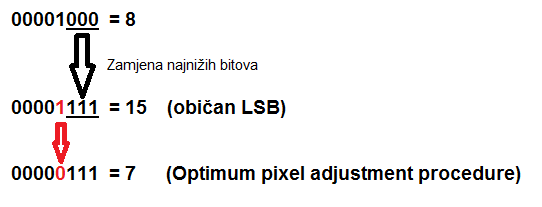
\includegraphics[scale=0.8]{images/LSB_cmp.png}}
\end{figure}
\paragraph{}
Kao što je već spomenuto, \textit{LSB} steganografski postupci se mogu koristiti i na \textit{GIF} slikama jer one koriste lossless kompresiju (konkretno, \textit{LZW} kompresiju), ali valja biti oprezan. Problem je u tome što \textit{GIF} slike spremaju različite boje koje se koriste u takozvanu tablicu "paletu boja", gdje je svakoj boji dodijeljen indeks u toj tablici. U takvoj slici su svi pikseli definirani samo indeksom u toj paleti pa je bitno paziti jer bliski indeksi u paleti boja mogu rezultirati potpuno različitim bojama pa nije dobro izravno primjenjivati \textit{LSB} postupak. Taj problem se može riješiti tako da se sortiraju boje u paleti, što će dovesti do toga da slični indeksi rezultiraju sličnim bojama pa je onda moguće raditi običan LSB algoritam.
\paragraph{}
Drugi način za doskočiti ovom problemu je da uvodimo nove boje u paletu koje su vizualno slične već postojećim bojama u paleti. Ovo zahtijeva da je broj korištenih boja u paleti manji od maksimalnog broja boja pa je potrebno paziti u kakve slike skrivamo poruke. Još jedan način rješavanja ovog problema je da koristimo crno-bijele slike gdje imamo 256 različitih nijansi sive gdje je promjena u nijansama vrlo postepena i teža za uočiti.
\paragraph{}
Nadalje imamo još neke postupke iz slikovne domene, koje nazivamo \textit{mod} postupci. Često se koristi mod10 koji svakom pikselu oduzme njegov ostatak pri dijeljenju sa 10 te mu nadoda bitove iz poruke, opet iz intervala [0,9]. Ovaj postupak je lakše za implementirati od običnog LSB algoritma te se dosta koristi pogotovo na crno-bijelim slikama. Rekonstrukcija poruke iz ovako kodirane slike se također lagano provodi: jednostavno iz svakog piksela izvadimo njegov ostatak pri dijeljenju sa 10.
\paragraph{}
Još jedan predstavnik steganografskih postupaka iz slikovne domene je \textit{patchwork}. Taj postupak daje pseudoslučajni, statistički model koji višestruko skriva istu poruku na slici. Radi na principu da odabire slučajno po dva područja (\textit{patch}-a) na slici te jednome poveća intenzitet za neku konstantu, dok drugome smanji za konstantu. Time se osigurava da je očekivana promjena intenziteta jednaka 0 što uvelike pomaže da postupak bude visoko transparentan. Ono što je dobro kod ovog algoritma je što je otporan na neke transformacije slike kao što je npr rezanje dijelova slike ili rotacije, upravo zato što se ista poruka kodira na više mjesta na slici. S druge strane, ta činjenica dovodi do loše strane ovog pristupa a to je mali kapacitet. Zato se ovaj pristup koristi samo kada treba prenijeti male poruke.
\paragraph{}
Osvrnut ćemo se još malo na format slika \textit{JPEG}. Taj format je jedan od najkorištenijih formata općenito te su osmišljeni brojni steganografski postupci koji dobro rade upravo za ovaj format. \textit{JPEG} slike koriste lossy kompresiju i to na način da se izvede prvo diskretna kosinusna transformacija (\textit{DCT}) nad slikom te se spremaju koeficijenti koji se dobiju, a nakon toga se Huffmanovim kodiranjem komprimiraju ti koeficijenti. Rekonstrukcijom iz tih koeficijenata se dobiva dobra (ali ipak ne savršena) aproksimacija originalne slike. Zato što je kompresija \textit{lossy}, algoritmi koje smo dosad spomenuli ne mogu se primjeniti direktno na ovom formatu slika, ali je moguće primjeniti \textit{LSB} nad samim koeficijentima prije Huffmanovog kodiranja, jer će slični koeficijenti dati slične slike, a sami Huffmanov postupak je lossless kompresija što znači da će se poruka sačuvati.
\paragraph{}
Osim pristupa iz porodice \textit{LSB} algoritama, pogledat ćemo i neke postupke iz transformacijske domene. Postupci iz transformacijske domene su općenito robusniji od onih iz slikovne domene pa su jako korisni u slučajevima kada je slika podvrgnuta raznim transformacijama jer su relativno otporni na promjene u kodiranoj slici. Također, ovi postupci općenito imaju i veliki kapacitet te je moguće sakriti čak cijelu sliku unutar druge slike.
\paragraph{}
Jedan od tih postupaka je takozvani \textit{Spread-spectrum} postupak. On spada i u slikovnu domenu i u transformacijsku, ovisno o implementaciji. Originalno se koristi za ubacivanje tajnih zvučnih poruka u zvučne signale, ali se isti princip može primjeniti i na slikama. Algoritam se temelji na tome da se informacija koja se želi sakriti prikaže kao signal definiran na uskom području frekvencija i koji je općenito velike snage. Zatim se taj signal rastegne preko većeg raspona frekvencija, a time se i snaga smanji. Takav signal male snage će zapravo biti šum koji možemo ubaciti u drugi signal. Zbog niske snage, naša poruka će biti dobro skrivena(zagušena) i neće se čuti praktički nikakva razlika u odnosu na originalni signal. Kada signal dođe na odredište, poruka se može izvaditi iz signala korištenjem raznih filtera.  Slika \ref{transfrom} prikazuje transformaciju poruke u signal male snage i velikog raspona frekvencija.
\begin{figure}
\caption{Transformacija tajne poruke u signal male snage}
\label{transfrom}
\centerline{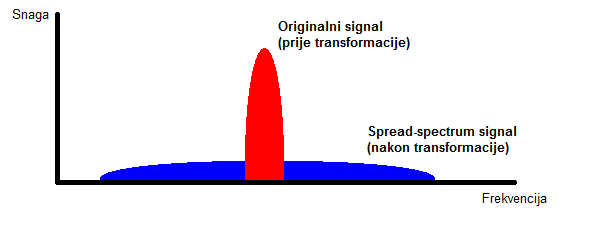
\includegraphics[scale=0.8]{images/transformation.png}}
\end{figure}
\paragraph{}
Jedni od najpoznatijih postupaka iz transformacijske domene su postupci koji se temelje na diskretnim transformacijama signala/slika. Konkretno, tu se koriste razne diskretne transformacije: kosinusna, Fourierova, transformacija valića itd. Ti postupci imaju veliki kapacitet i jako su povoljni za skrivanje slika unutar drugih slika. Funkcioniraju tako da se zbroje transformacije od originalne i skrivene slike putem enkodera te se iz tog zbroja izvuče slika koja se šalje. Zatim se na primateljevom kraju ta slika opet kombinira sa originalnom kako bi se mogao izvući onaj dio transformacije koji odgovara skrivenoj poruci. Pomoću inverzne diskretne transformacije se skrivena slika zatim rekonstruira. Slika \ref{dwt} prikazuje model steganografskog postupka koji se temelji na diskretnoj transformaciji valića (\textit{Discrete Wavelet Transform}).
\begin{figure}
\caption{Model steganografskog postupka temeljen na diskretnoj transformaciji valića (\textit{DWT})}
\label{dwt}
\centerline{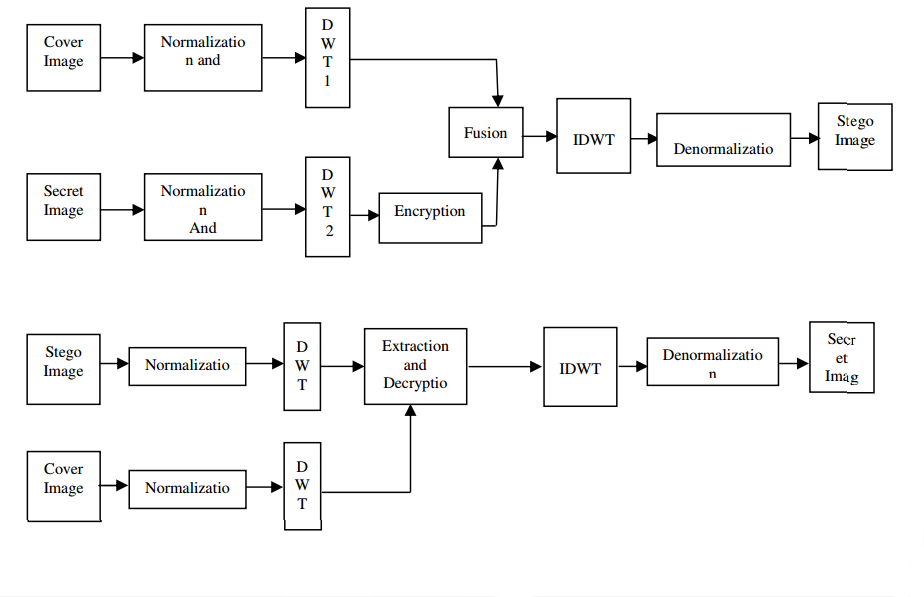
\includegraphics[scale=0.6]{images/dwt.png}}
\end{figure}
\paragraph{}
Opisali smo neke od brojnih steganografskih postupaka i pokazali u kojim situacijama se koriste. Svaki od tih postupaka ima svoje dobre strane i mane stoga je potrebno ovisno o problemu izabrati onaj pravi. U ovom projektu se za zadani problem koristi obični \textit{LSB} postupak zbog svoje jednostavnosti, a dovoljno je dobar za praktičnu primjenu, ali uvijek treba imati na umu i ostale postupke koji su nam na raspolaganju. 
%%end Backo
\section{Konceptualno rješenje zadatka}

\chapter{Postupak rješavanja zadataka}

\chapter{Ispitivanje rješenja}
\paragraph{}
Razvijeni sustav za steganografski postupak, kao i svi steganografski algoritmi, ograničen je količinom podataka koja se može upisati u neku sliku. Ova granica prvenstveno je određena veličinom slike, a određuju je i odabir kanala te najznačajniji bit do kojeg se upisuju podaci. Glavna ideja steganografskog algoritma jest upisati podatak u sliku bez velikog utjecaja na konačni izgled. Drugim riječima, izgled konačne slike uvjetovan je količinom podataka koji se u nju upisuju. Potrebno je pronaći dobre parametre steganografskog algoritma koji nude dobara kapacitet skrivenih podataka, a neznatno žrtvuju kvalitetu izvorne slike.
\paragraph{}
Parametri algoritma koji su podešavani u ispitivanju su:
\begin{itemize}
\item Najznačajniji bit do kojeg se slijedno upisuje podatak
\item RGB komponente u koje će se upisivati podaci
\end{itemize}
Algoritam \textit{Least Significant Bit(LSB)} upisivanje sadržaja započinje s bitovima najnižeg značaja. Razlog tome leži u tome što se izmjenom bita najmanjeg značaja piksel najmanje mijenja. Praktični primjer bio bi kada bismo odlučili mijenjati samo B(\textit{blue}) komponentu i to samo najniži bit svakog bajta. Za svaki piksel slike(3 komponente, svaka po 1 bajt) dobije se jedan bit prostora za skrivanje podataka. Općenito, količina podataka koja se može upisati($n_{data}$), u ovisnosti o broju komponenti za upisivanje $n_{components}$ i broja najnižih bitova svake odabrane komponente za upisivanje $n_{bits}$ te veličini(broju piksela) $n_{pixels}$ slike je:
\begin{equation}
\label{num_bits}
n_{data} = \floor{\cfrac{n_{pixels} \cdot n_{components} \cdot n_{bits}}{8}}
\tagaddtext{[B]}
\end{equation}
\paragraph{}
Udio veličine podataka $\eta$ koje je za dane parametre moguće upisati u sliku u odnosu na ukupnu veličinu slike je:
\begin{equation}
\label{eta}
\eta = \cfrac{n_{data}}{3 \cdot n_{pixels}} = \cfrac{n_{components} \cdot n_{bits}}{24}
\end{equation}
Povećanjem $\eta$ vizualna razlika između izvorne slike i slike obrađene steganografskim algoritmom, u našem slučaju \textit{LSB}-om, povećava se. U nastavku slijede rezultati ispitivanja odnosa izvorne i obrađene slike u ovisnosti o parametrima $n_{components}$ i $n_{bits}$.
\section{Ispitna baza}
\paragraph{}
Ispitivanje algoritma \textit{LSB} napravljeno je nad dvjema različitim slikama. Slika \ref{chart_original} korištena je kako bi se ispitala osjetljivost boja na postupak, dok bi slika \ref{pattern_original} trebala pokazati osjetljivost tekstura. Ispitni primjeri pripremljeni su u ovisnosti o parametrima $n_{components}$ i $n_{bits}$. Za obje izvorne slike algoritam je pokrenut za sve moguće kombinacije parametara. Parametar $n_{components}$ poprima vrijednosti iz $[1,3]$, pošto svaki piksel ima crvenu, zelenu i plavu komponentu boje. Parametar $n_{bits}$ poprima vrijednosti iz $[1,8]$, gdje se za svaki bajt koristi $n_{bits}$ bitova u koje se upisuje podatak. Ukupno postoje 24 moguća para parametara algoritma. Nadalje, za svaki ispitni primjer odabrana je najveća količina podataka moguća za dane parametre, te su generirani nizovi bitova nasumične vrijednosti. U idućem odjeljku slijede rezultati ispitivanja, koji vizualno prikazuju promjenu kvalitete slike u ovisnosti o parametrima algoritma.
\begin{center}
\begin{figure}[ht]
	\caption{Izvorna slika jednostavnih boja, bez teksture}
	\label{chart_original}
	\centerline{
	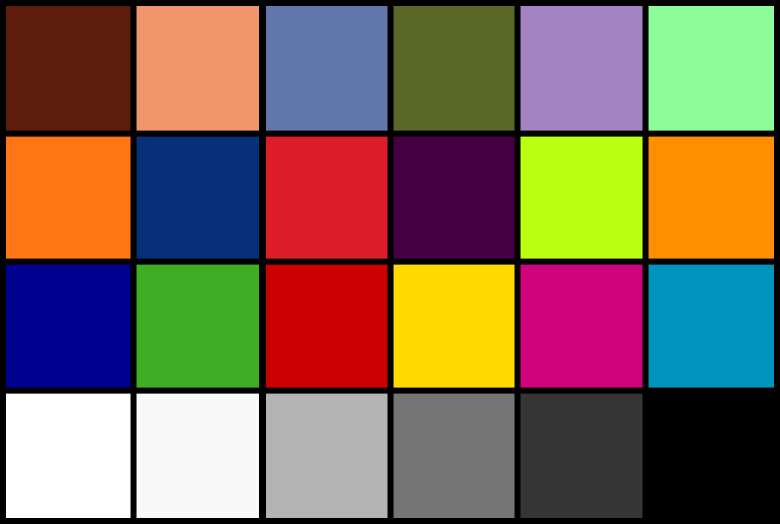
\includegraphics[scale=0.4]{../benchmark_results/color_chart/original.png}	
	}
\end{figure}
\end{center}

\begin{center}

\begin{figure}[ht]
	\caption{Izvorna slika s teksturom}
	\label{pattern_original}
	\centerline{
	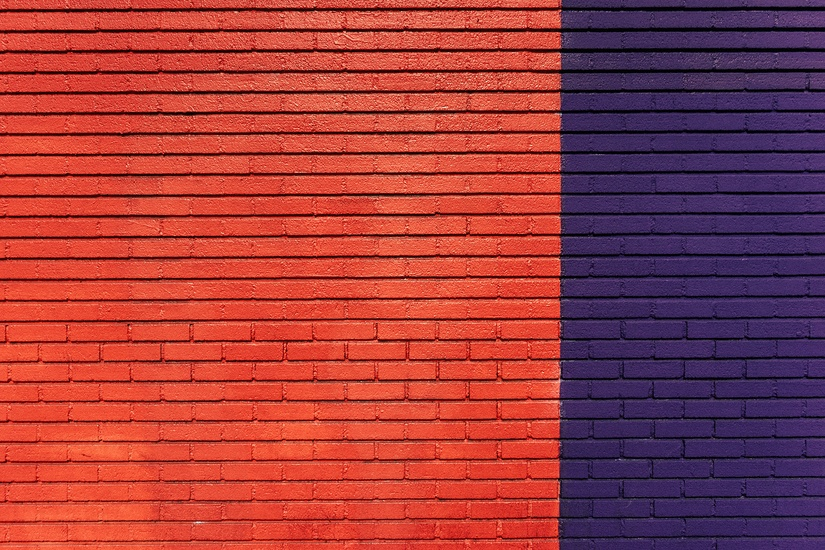
\includegraphics[scale=0.4]{../benchmark_results/pattern/pattern_original.jpg}	
	}
\end{figure}
\end{center}

\section{Rezultati ispitivanja}
\paragraph{}
Tablice \ref{table_chart} i \ref{pattern_original} prikazuju obređene slike algoritmom \textit{LSB} za vrijednosti parametara $n_{components}$ i $n_{bits}$. Treći stupac, $\eta$, prikazuje udio upisanih podataka u ukupnoj veličini slike.
\begin{center}
\begin{longtable}{|c|c|c|c|}
\caption{Osjetljivost kvalitete slike jednostavnih boja na \textit{LSB} u ovisnosti o parametrima $n_{components}$ i $n_{bits}$}\\
\hline
\textbf{$n_{components}$} & \textbf{$n_{bits}$} & \textbf{$\eta$} & \textbf{Slika}\\
\hline
\label{table_chart}
\endfirsthead
\multicolumn{4}{c}%
{\tablename\ \thetable\ -- \textit{Nastavljeno s prethodne strane}} \\
\hline
\textbf{$n_{components}$} & \textbf{$n_{bits}$} & \textbf{$\eta$} & \textbf{Slika}\\
\hline
\endhead
\hline \multicolumn{4}{r}{\textit{Nastavlja se na idućoj strani}} \\
\endfoot
\hline
\endlastfoot
1 & 1 &4\% & 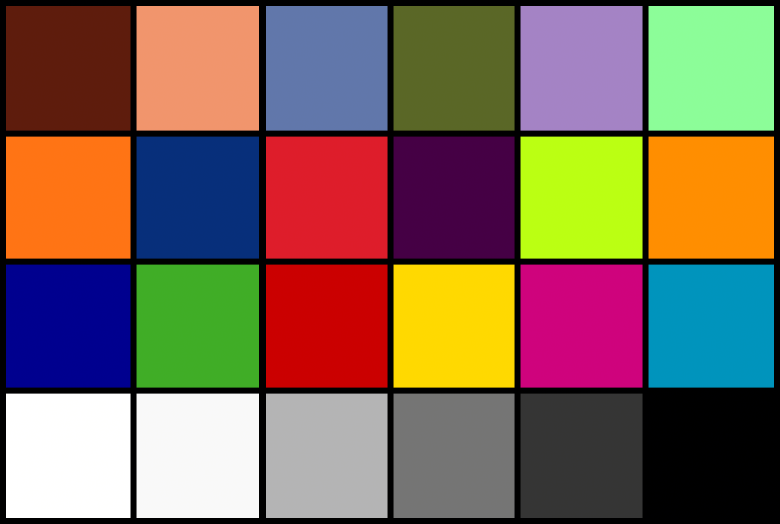
\includegraphics[scale=0.3]{../benchmark_results/color_chart/1_components-1_bits.png} \\
1 & 2 &8\% & 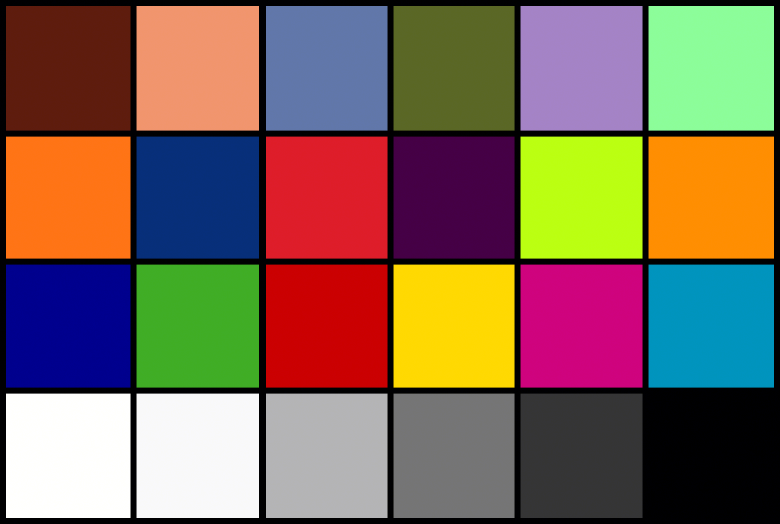
\includegraphics[scale=0.3]{../benchmark_results/color_chart/1_components-2_bits.png} \\
1 & 3 &12\% & 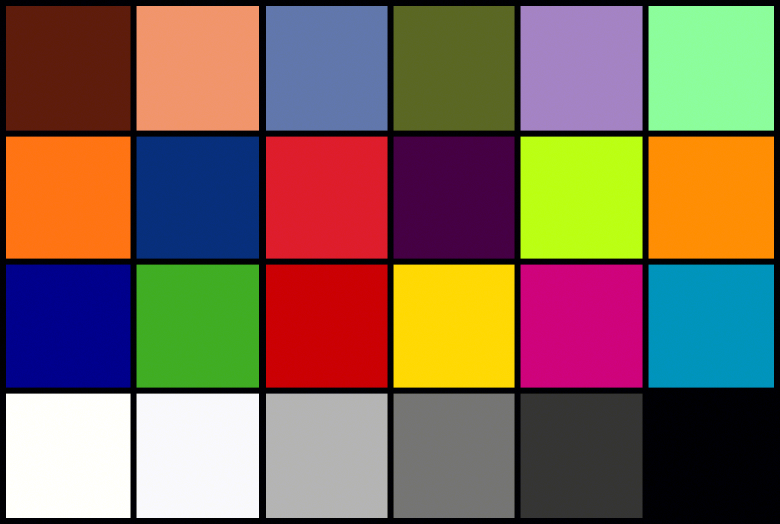
\includegraphics[scale=0.3]{../benchmark_results/color_chart/1_components-3_bits.png} \\
1 & 4 &17\% & 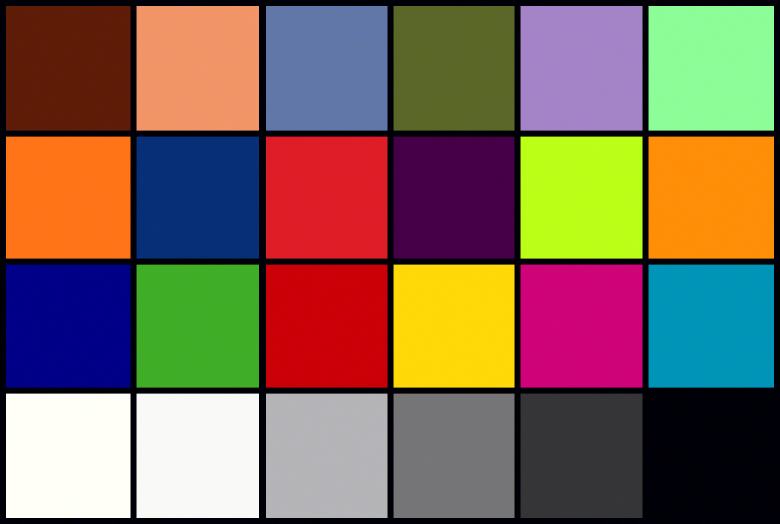
\includegraphics[scale=0.3]{../benchmark_results/color_chart/1_components-4_bits.png} \\
1 & 5 &21\% & 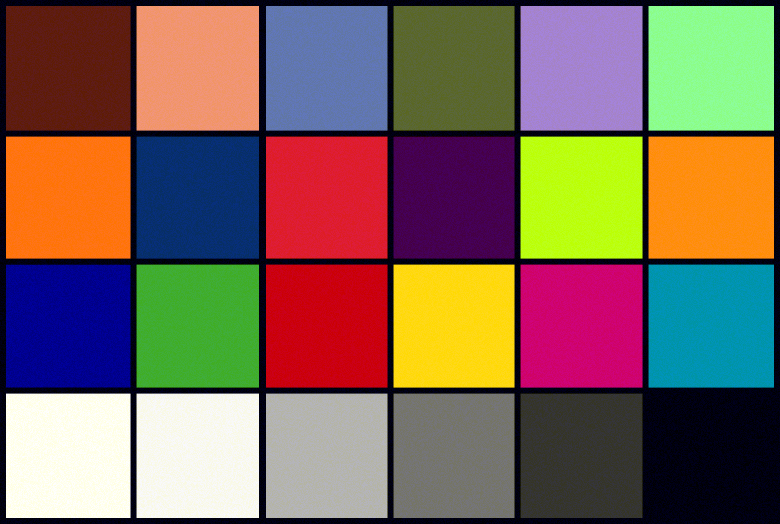
\includegraphics[scale=0.3]{../benchmark_results/color_chart/1_components-5_bits.png} \\
1 & 6 &25\% & 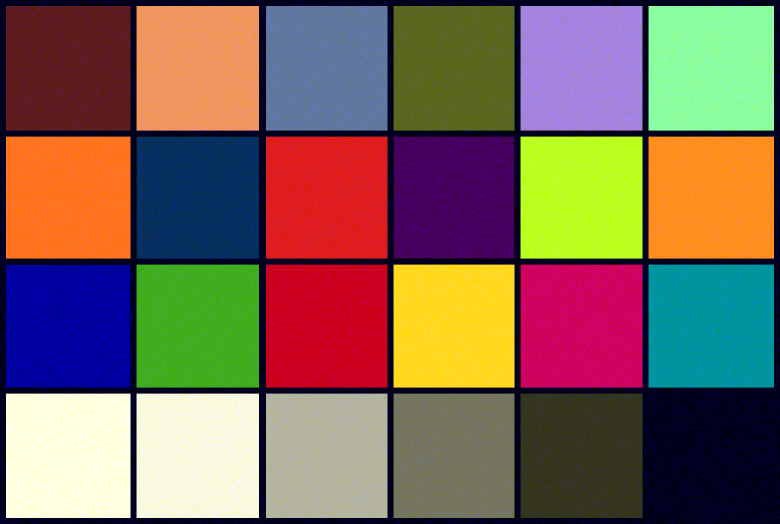
\includegraphics[scale=0.3]{../benchmark_results/color_chart/1_components-6_bits.png} \\
1 & 7 &29\% & 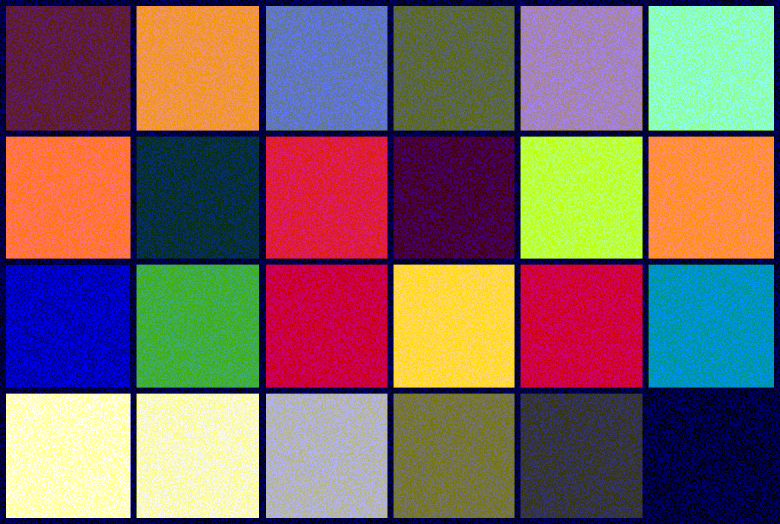
\includegraphics[scale=0.3]{../benchmark_results/color_chart/1_components-7_bits.png} \\
1 & 8 &33\% & 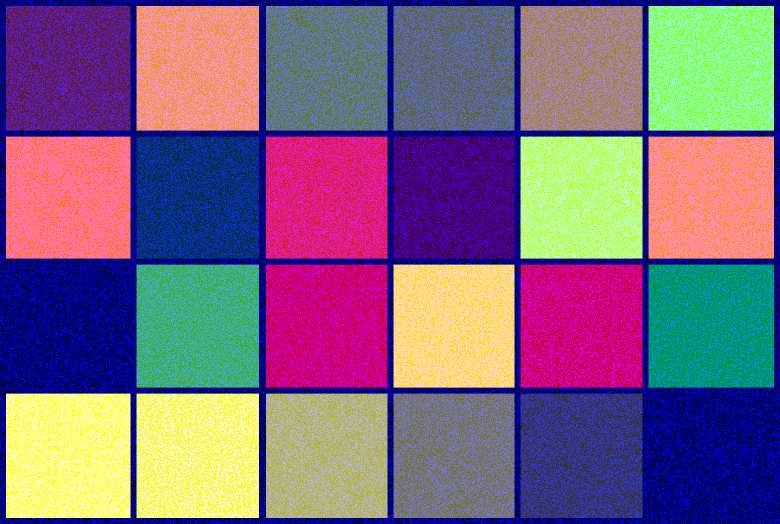
\includegraphics[scale=0.3]{../benchmark_results/color_chart/1_components-8_bits.png} \\
2 & 1 &8\% & 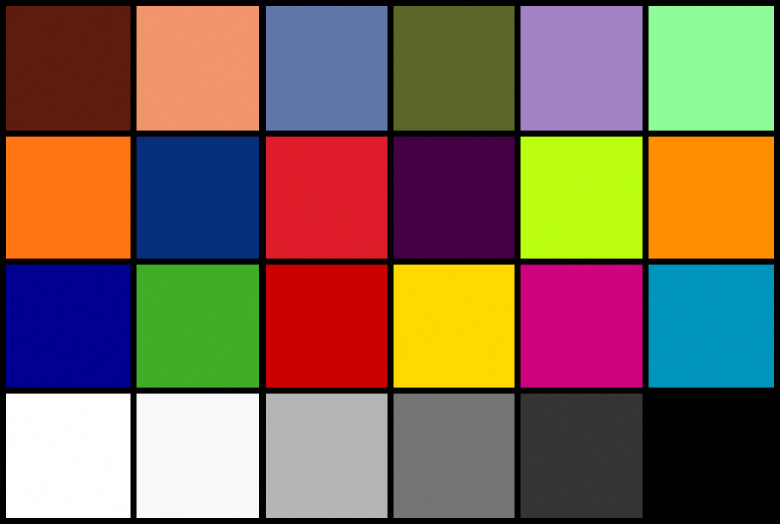
\includegraphics[scale=0.3]{../benchmark_results/color_chart/2_components-1_bits.png} \\
2 & 2 &12\% & 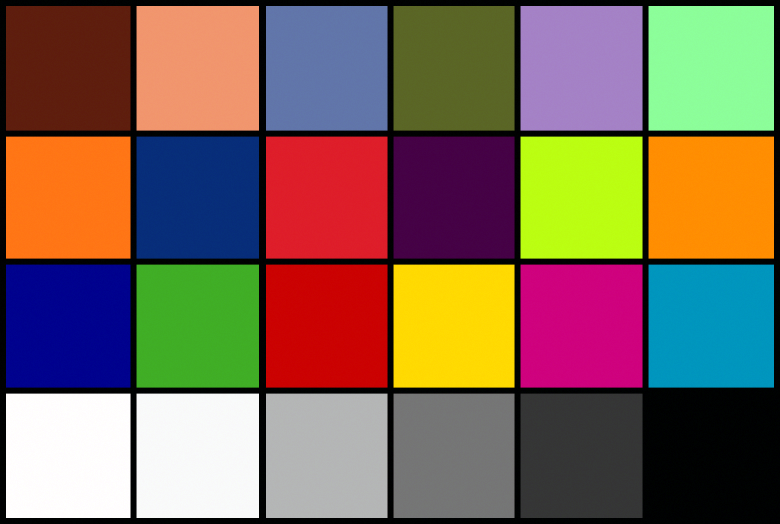
\includegraphics[scale=0.3]{../benchmark_results/color_chart/2_components-2_bits.png} \\
2 & 3 &25\% & 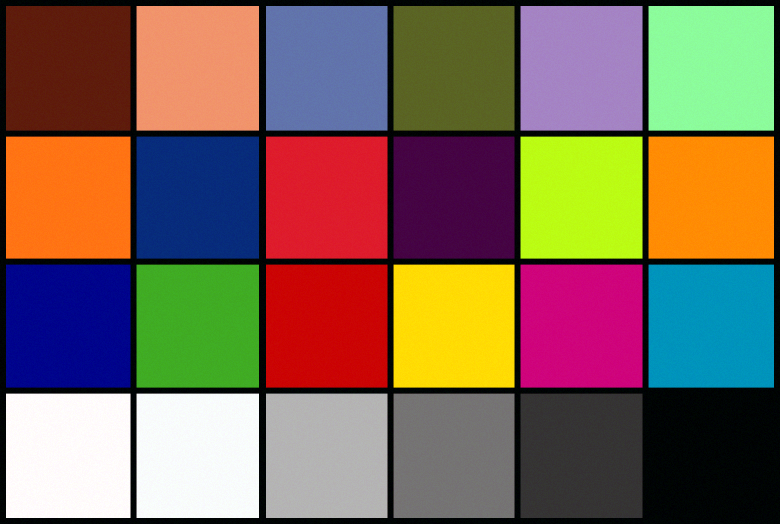
\includegraphics[scale=0.3]{../benchmark_results/color_chart/2_components-3_bits.png} \\
2 & 4 &33\% & 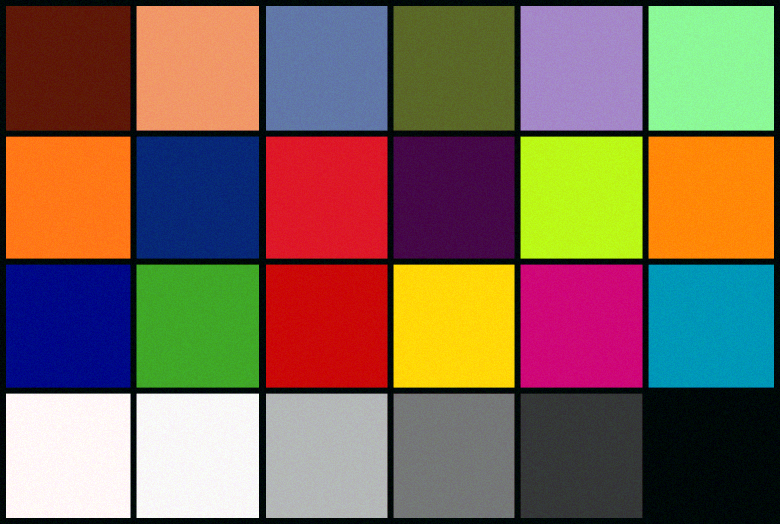
\includegraphics[scale=0.3]{../benchmark_results/color_chart/2_components-4_bits.png} \\
2 & 5 &42\% & 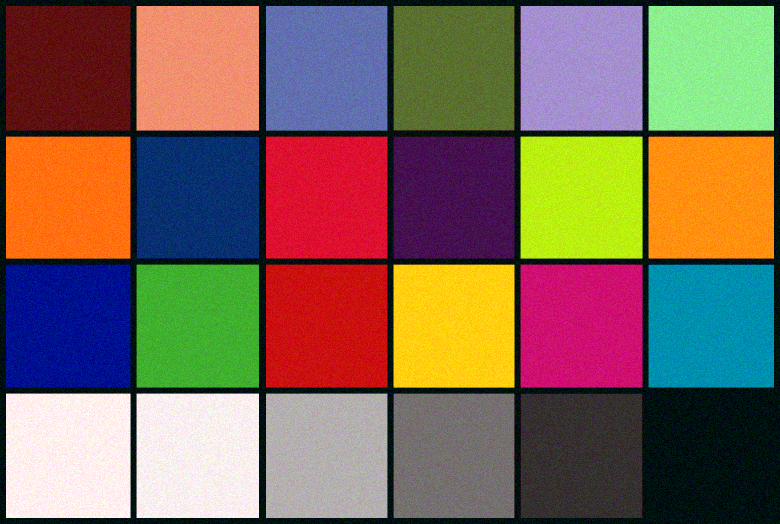
\includegraphics[scale=0.3]{../benchmark_results/color_chart/2_components-5_bits.png} \\
2 & 6 &50\% & 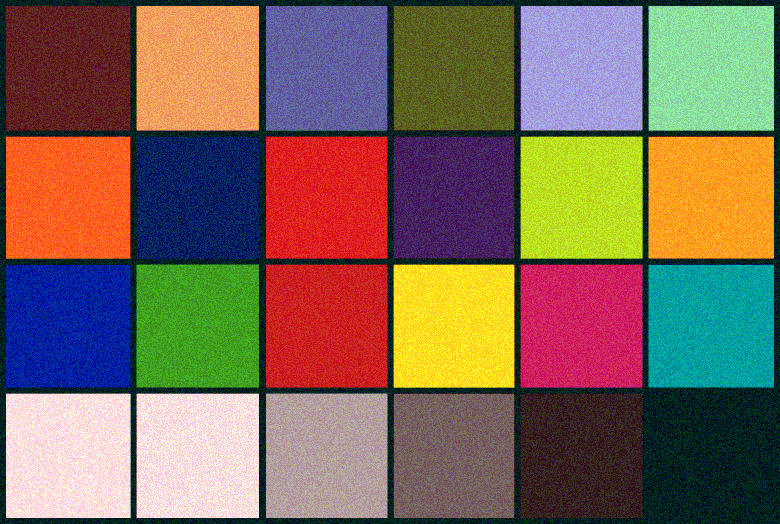
\includegraphics[scale=0.3]{../benchmark_results/color_chart/2_components-6_bits.png} \\
2 & 7 &58\% & 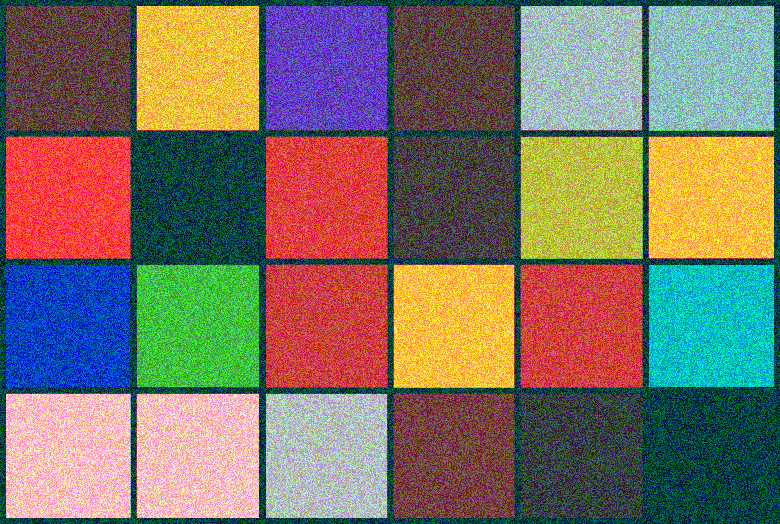
\includegraphics[scale=0.3]{../benchmark_results/color_chart/2_components-7_bits.png} \\
2 & 8 &67\% & 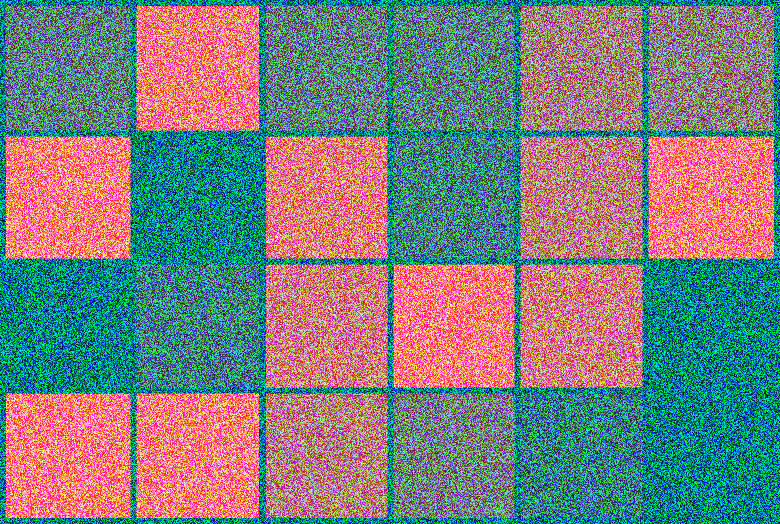
\includegraphics[scale=0.3]{../benchmark_results/color_chart/2_components-8_bits.png} \\
3 & 1 &12\% & 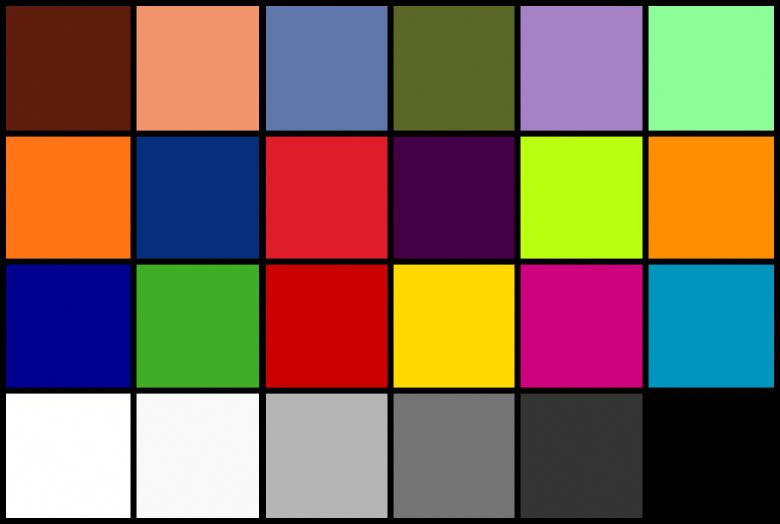
\includegraphics[scale=0.3]{../benchmark_results/color_chart/3_components-1_bits.png} \\
3 & 2 &25\% & 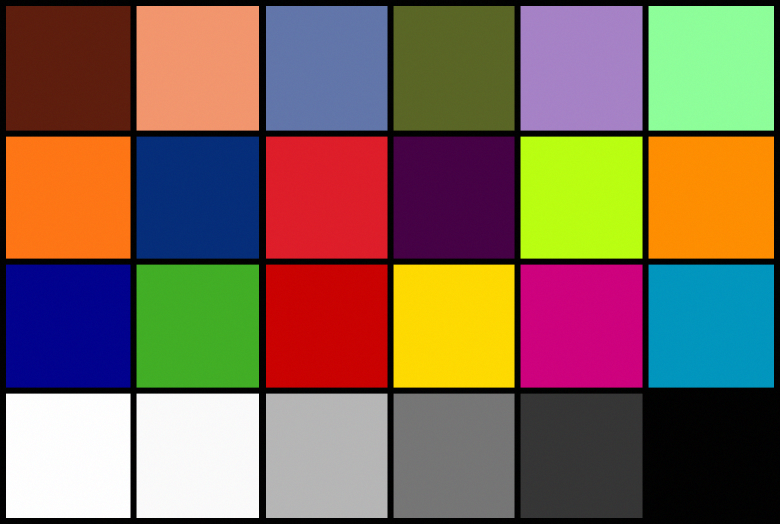
\includegraphics[scale=0.3]{../benchmark_results/color_chart/3_components-2_bits.png} \\
3 & 3 &38\% & 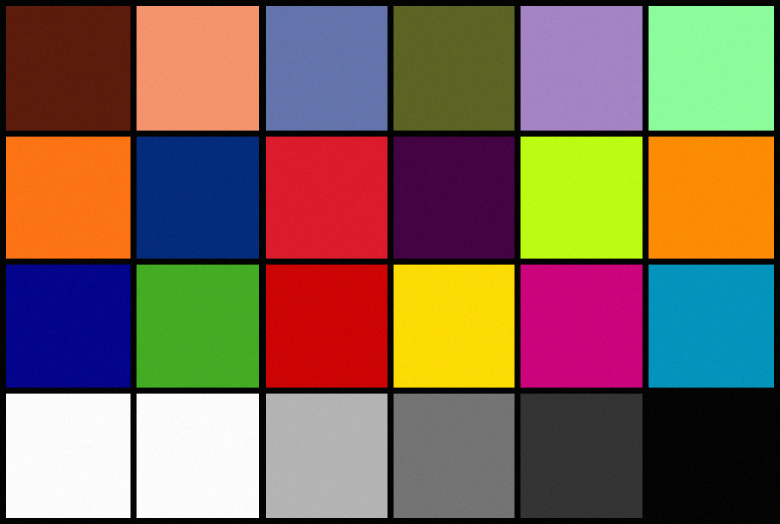
\includegraphics[scale=0.3]{../benchmark_results/color_chart/3_components-3_bits.png} \\
3 & 4 &50\% & 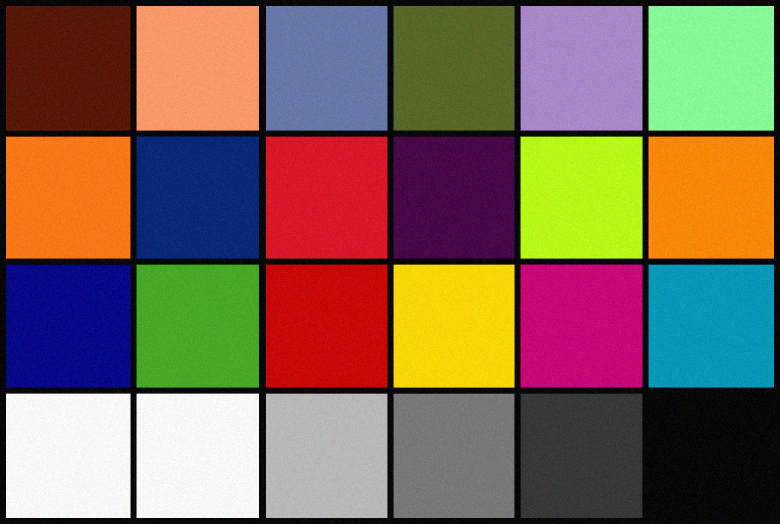
\includegraphics[scale=0.3]{../benchmark_results/color_chart/3_components-4_bits.png} \\
3 & 5 &62\% & 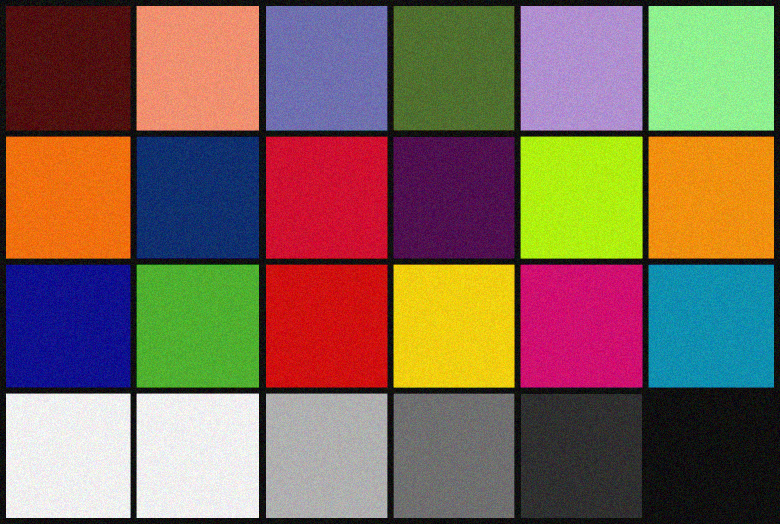
\includegraphics[scale=0.3]{../benchmark_results/color_chart/3_components-5_bits.png} \\
3 & 6 &75\% & 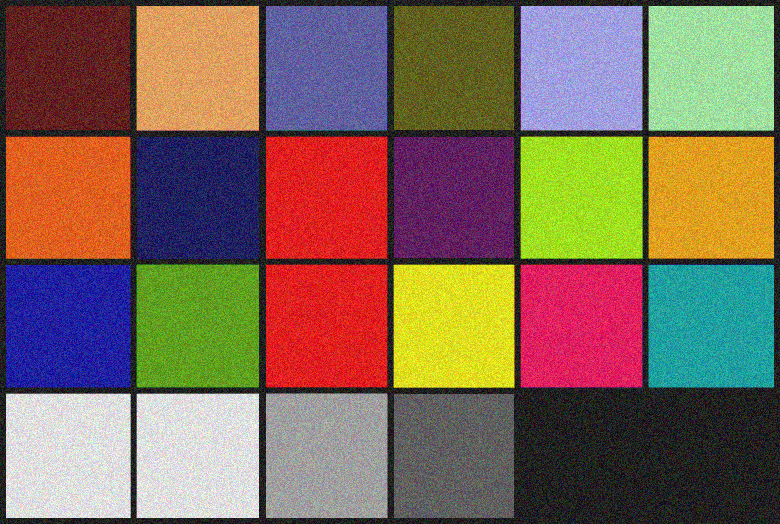
\includegraphics[scale=0.3]{../benchmark_results/color_chart/3_components-6_bits.png} \\
3 & 7 &88\% & 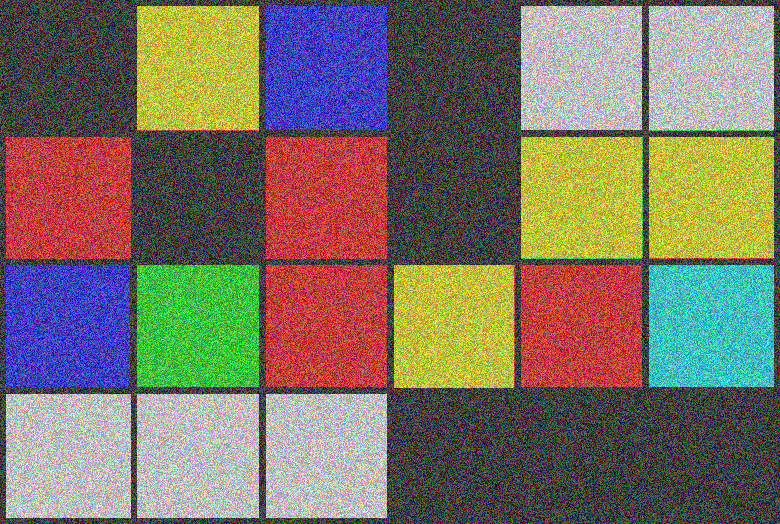
\includegraphics[scale=0.3]{../benchmark_results/color_chart/3_components-7_bits.png} \\
3 & 8 &100\% & 
\includegraphics[scale=0.3]{../benchmark_results/color_chart/3_components-8_bits.png} \\
\end{longtable}
\end{center}

\begin{center}
\begin{longtable}{|c|c|c|c|}
\caption{Osjetljivost kvalitete slike tekstura na \textit{LSB} u ovisnosti o parametrima $n_{components}$ i $n_{bits}$}\\
\hline
\textbf{$n_{components}$} & \textbf{$n_{bits}$} & \textbf{$\eta$} & \textbf{Slika}\\
\hline
\label{table_pattern}
\endfirsthead
\multicolumn{4}{c}%
{\tablename\ \thetable\ -- \textit{Nastavljeno s prethodne strane}} \\
\hline
\textbf{$n_{components}$} & \textbf{$n_{bits}$} & \textbf{$\eta$} & \textbf{Slika}\\
\hline
\endhead
\hline \multicolumn{4}{r}{\textit{Nastavlja se na idućoj strani}} \\
\endfoot
\hline
\endlastfoot
1 & 1 &4\% & 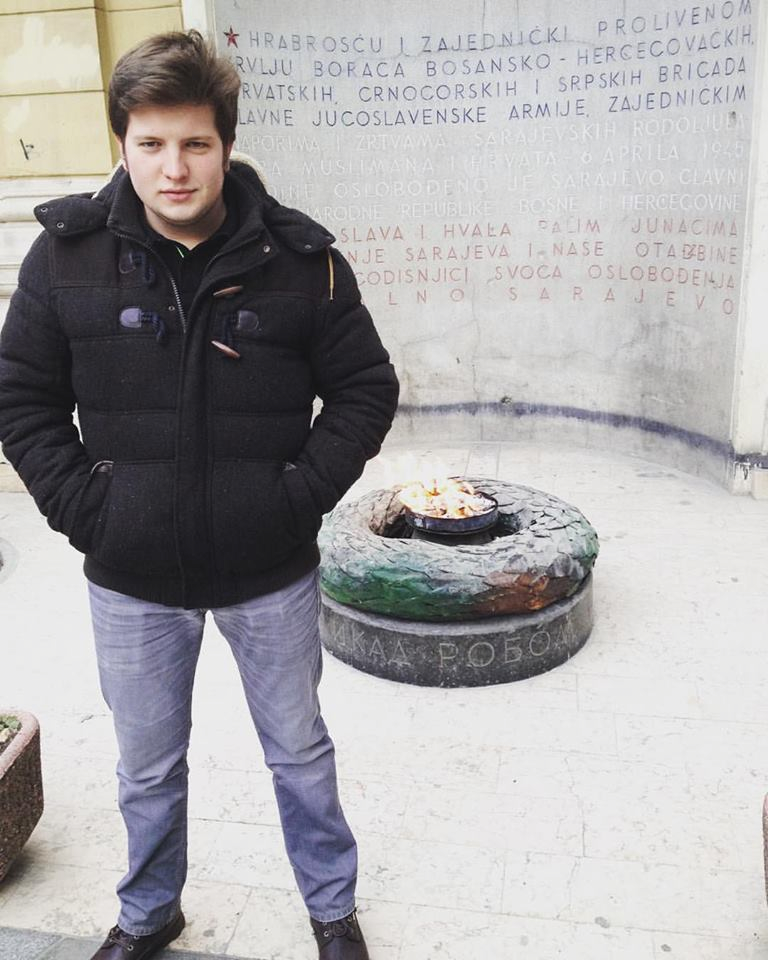
\includegraphics[scale=0.3]{../benchmark_results/pattern/1_components-1_bits.png} \\
1 & 2 &8\% & 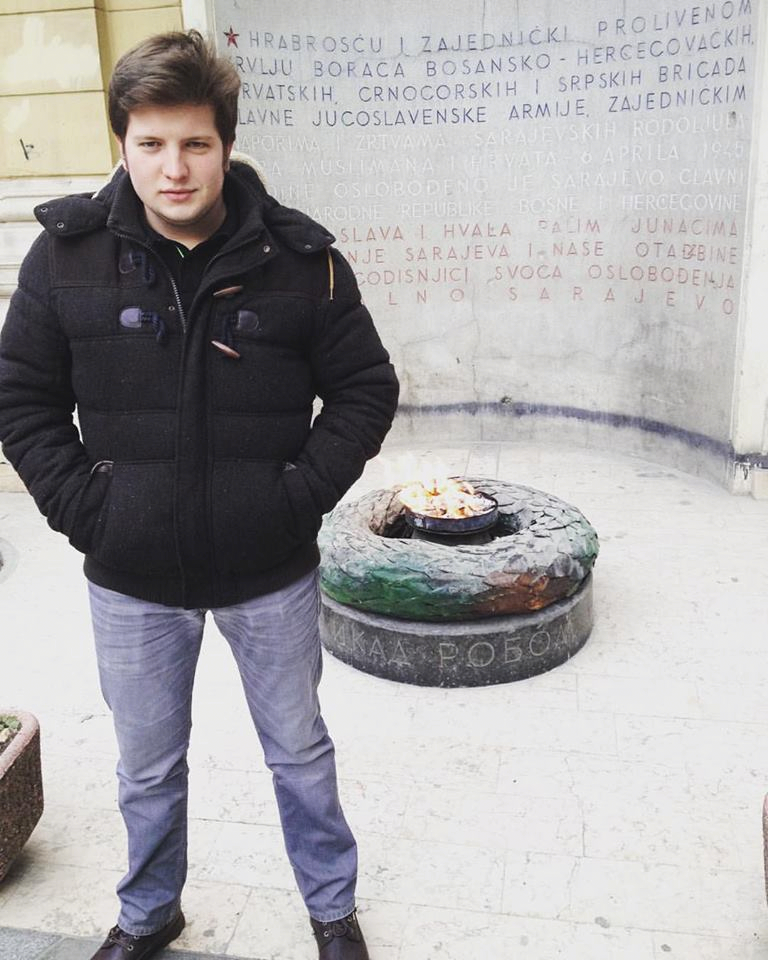
\includegraphics[scale=0.3]{../benchmark_results/pattern/1_components-2_bits.png} \\
1 & 3 &12\% & 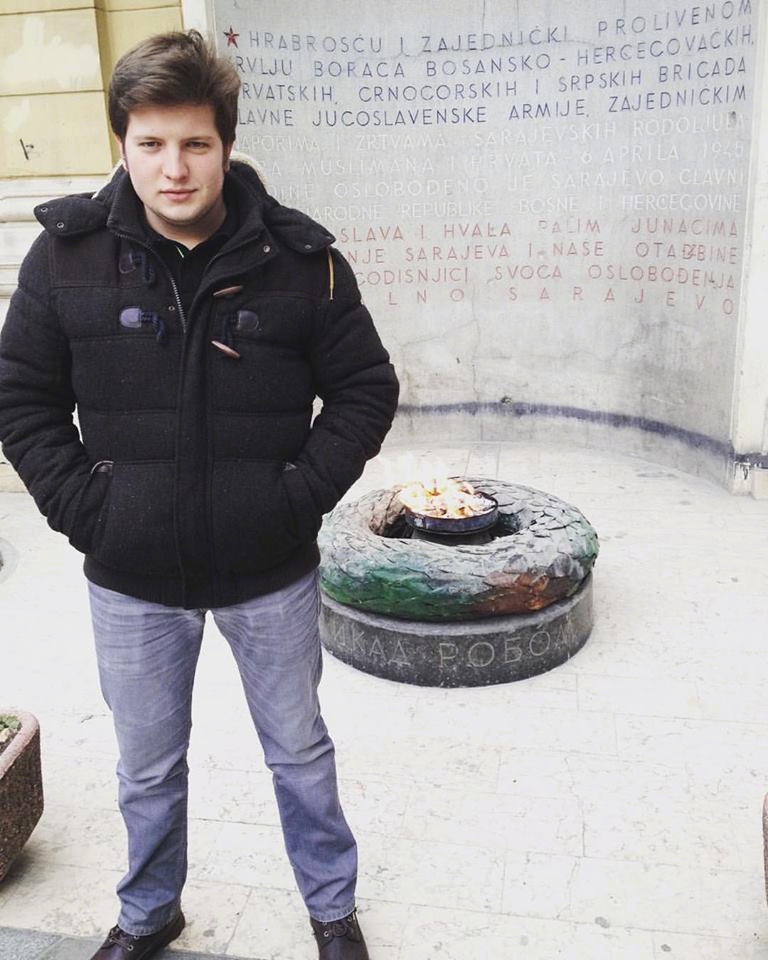
\includegraphics[scale=0.3]{../benchmark_results/pattern/1_components-3_bits.png} \\
1 & 4 &17\% & 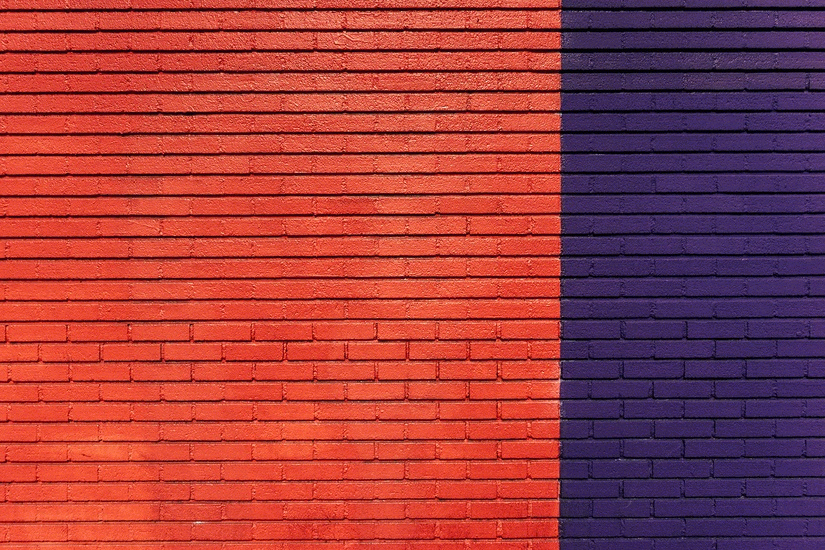
\includegraphics[scale=0.3]{../benchmark_results/pattern/1_components-4_bits.png} \\
1 & 5 &21\% & 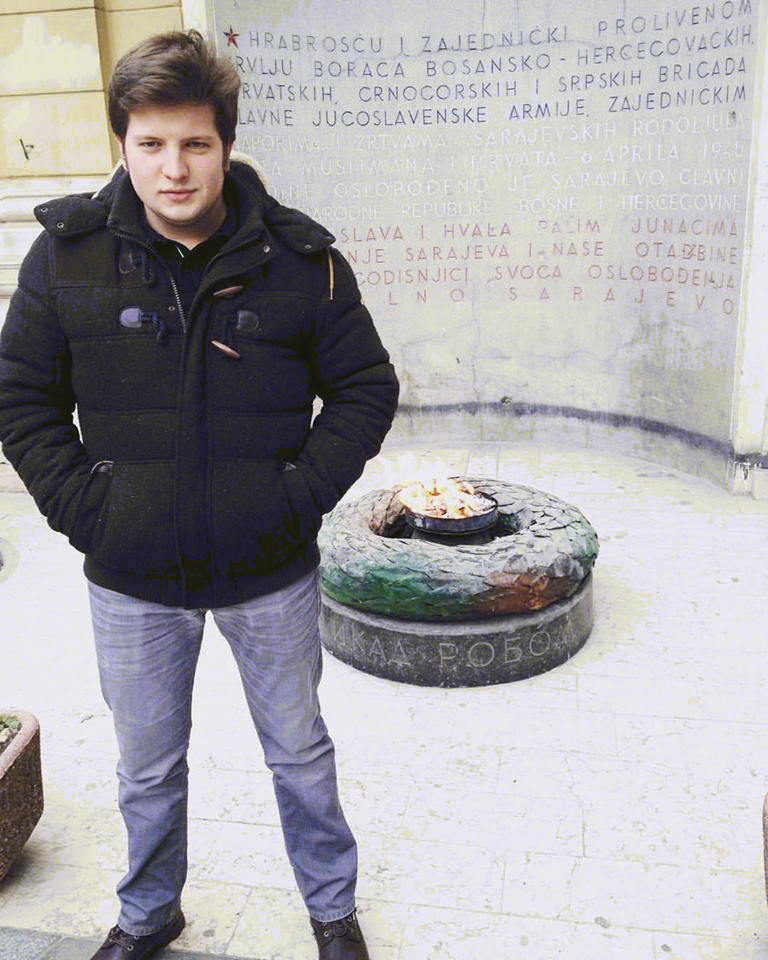
\includegraphics[scale=0.3]{../benchmark_results/pattern/1_components-5_bits.png} \\
1 & 6 &25\% & 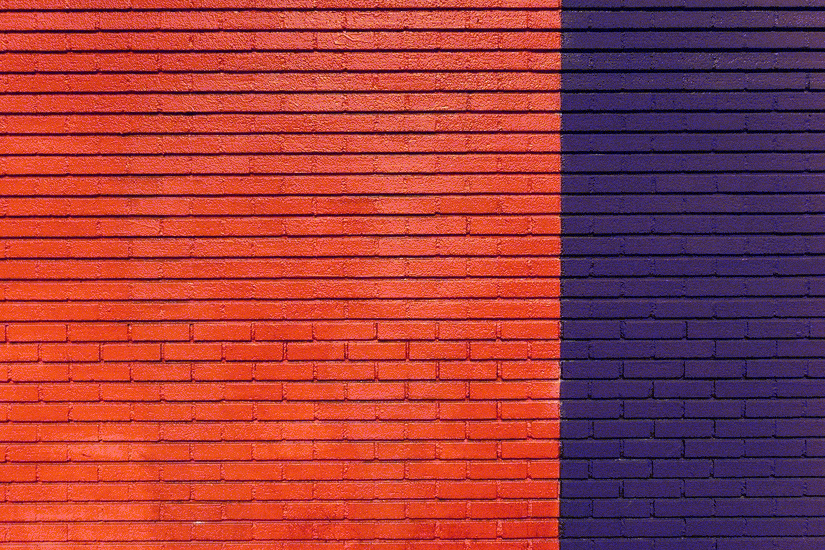
\includegraphics[scale=0.3]{../benchmark_results/pattern/1_components-6_bits.png} \\
1 & 7 &29\% & 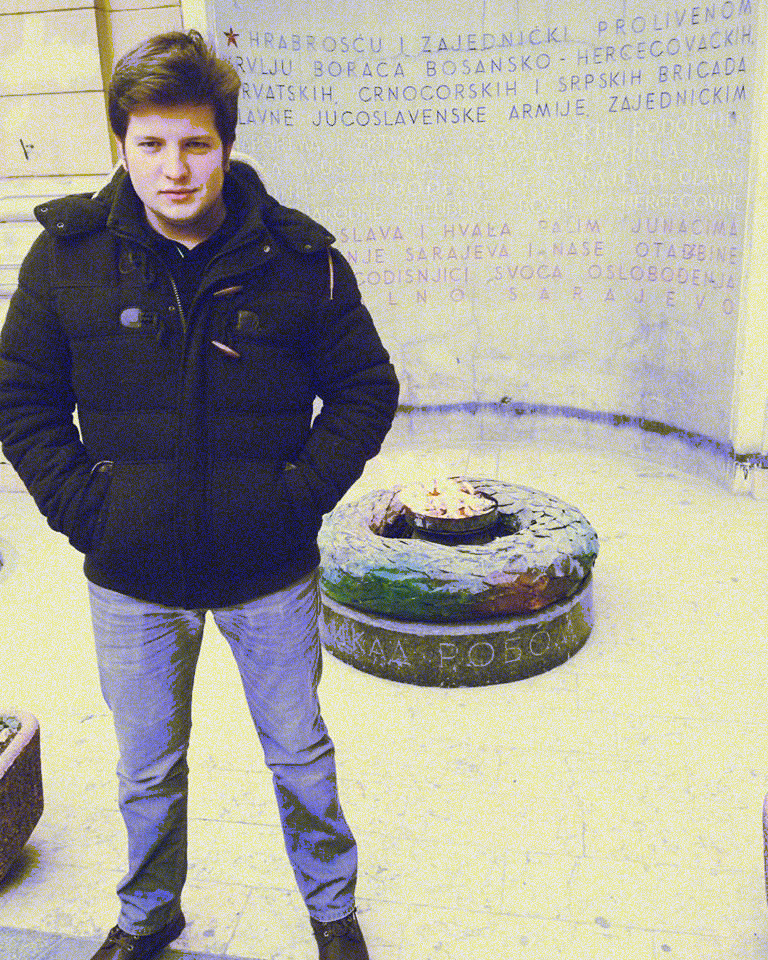
\includegraphics[scale=0.3]{../benchmark_results/pattern/1_components-7_bits.png} \\
1 & 8 &33\% & 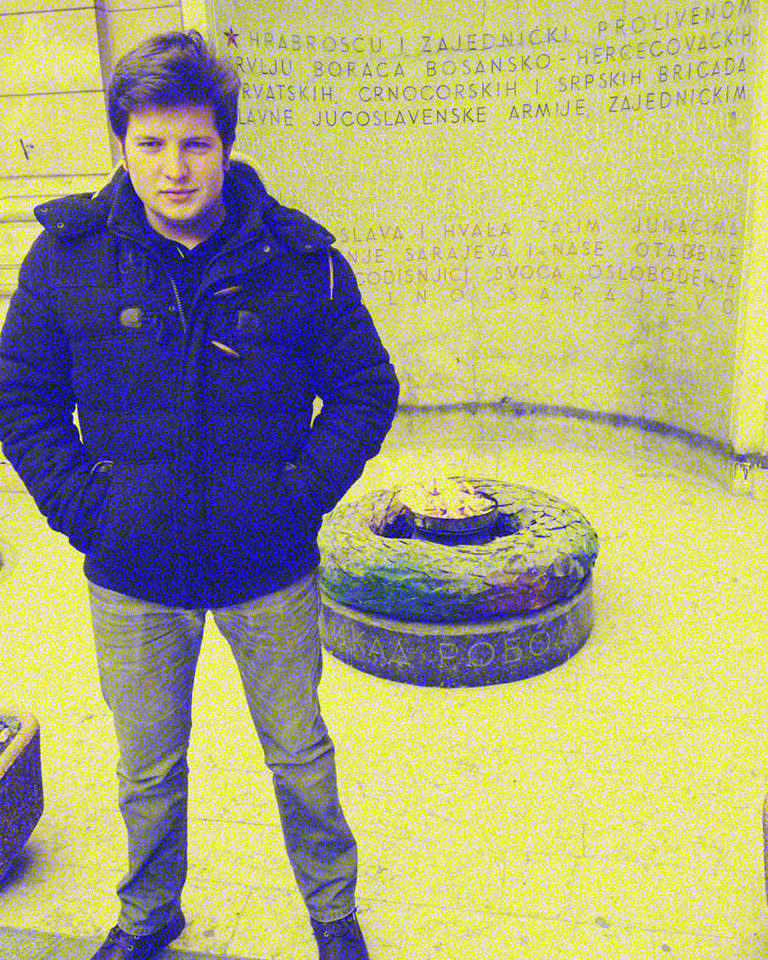
\includegraphics[scale=0.3]{../benchmark_results/pattern/1_components-8_bits.png} \\
2 & 1 &8\% & 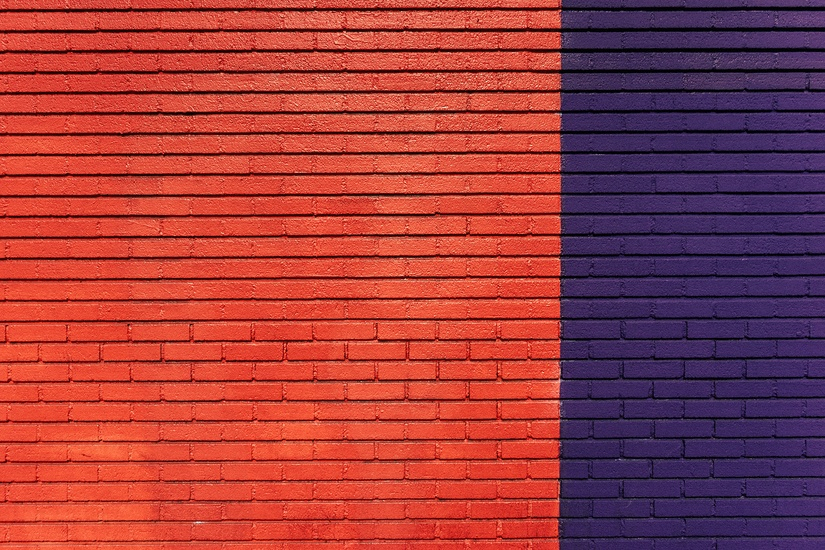
\includegraphics[scale=0.3]{../benchmark_results/pattern/2_components-1_bits.png} \\
2 & 2 &12\% & 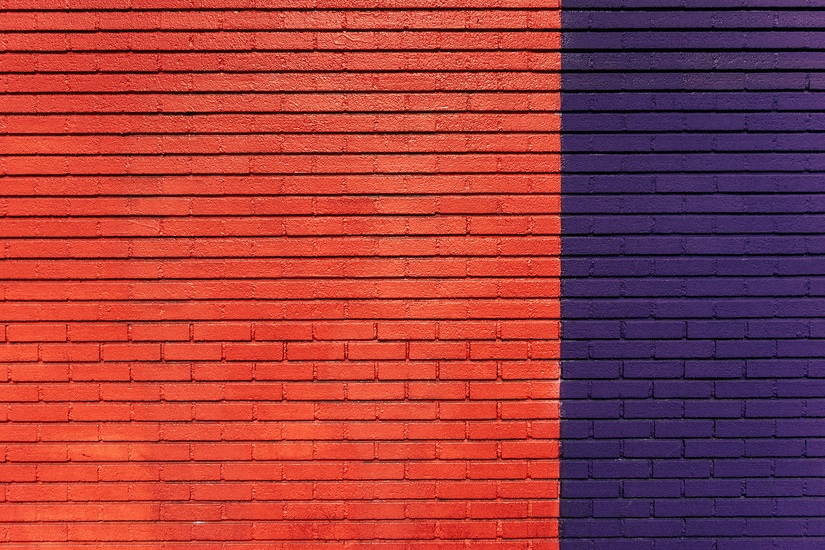
\includegraphics[scale=0.3]{../benchmark_results/pattern/2_components-2_bits.png} \\
2 & 3 &25\% & 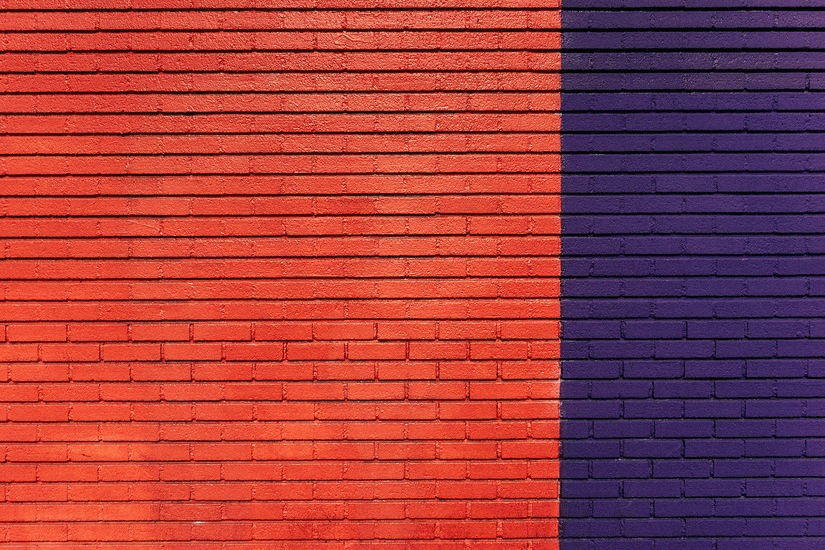
\includegraphics[scale=0.3]{../benchmark_results/pattern/2_components-3_bits.png} \\
2 & 4 &33\% & 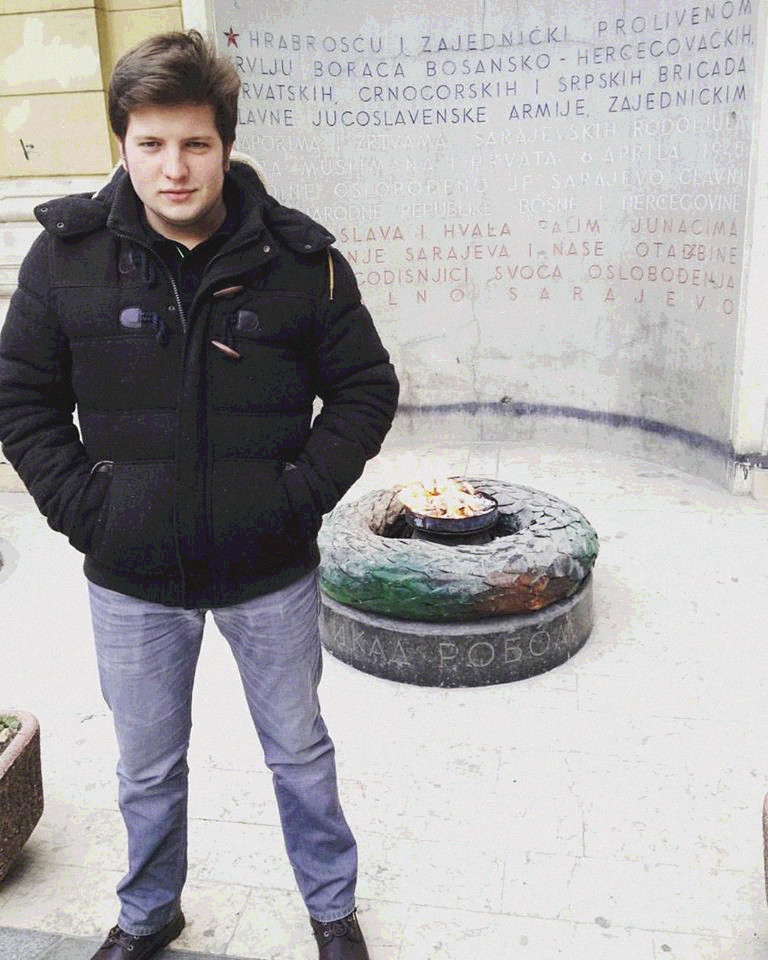
\includegraphics[scale=0.3]{../benchmark_results/pattern/2_components-4_bits.png} \\
2 & 5 &42\% & 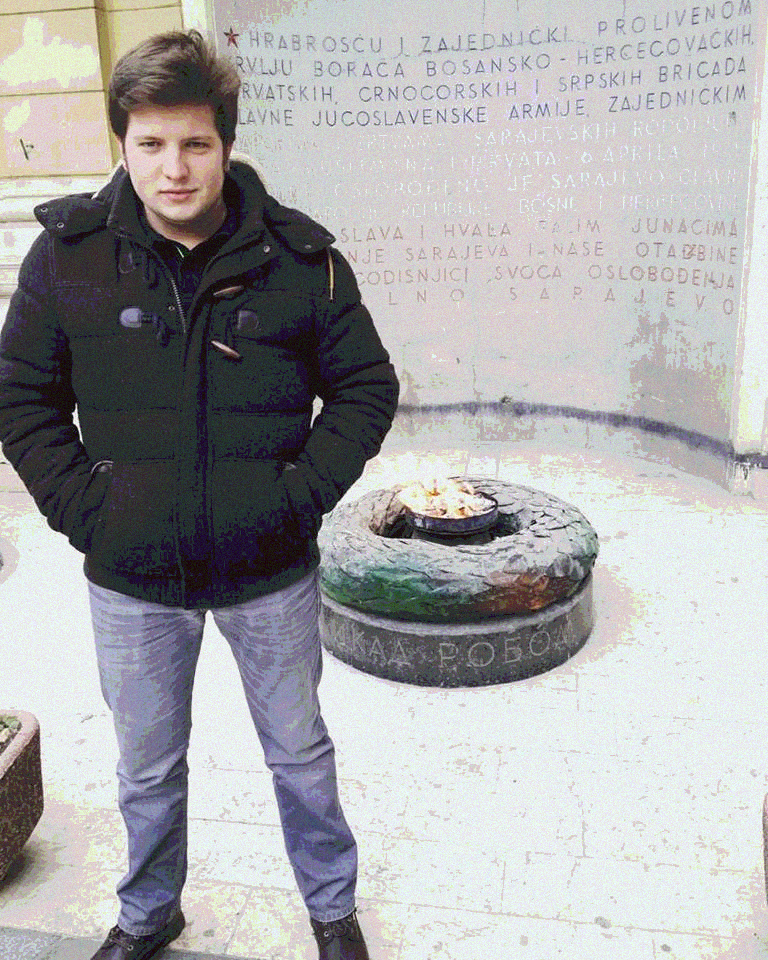
\includegraphics[scale=0.3]{../benchmark_results/pattern/2_components-5_bits.png} \\
2 & 6 &50\% & 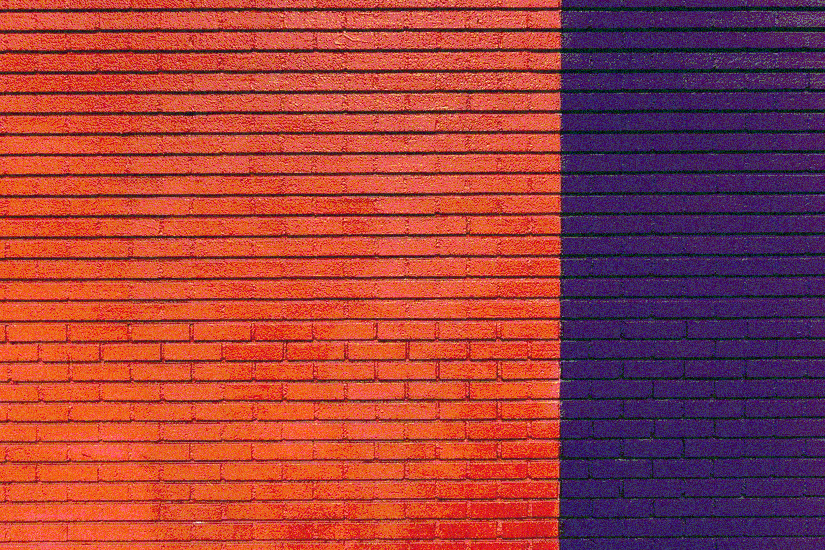
\includegraphics[scale=0.3]{../benchmark_results/pattern/2_components-6_bits.png} \\
2 & 7 &58\% & 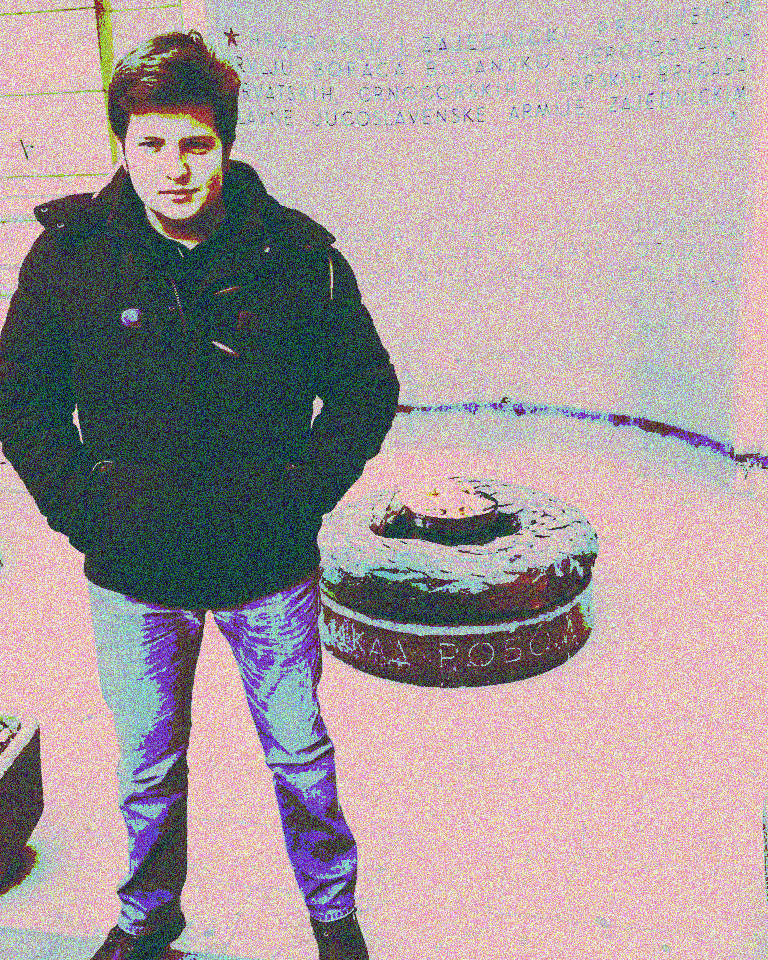
\includegraphics[scale=0.3]{../benchmark_results/pattern/2_components-7_bits.png} \\
2 & 8 &67\% & 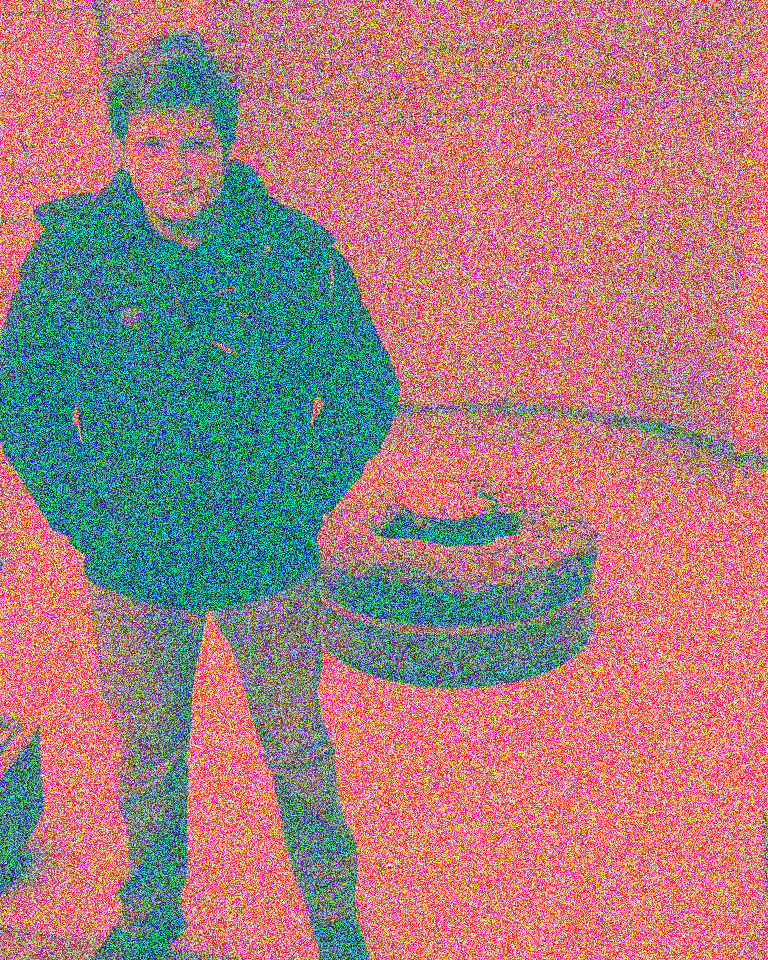
\includegraphics[scale=0.3]{../benchmark_results/pattern/2_components-8_bits.png} \\
3 & 1 &12\% & 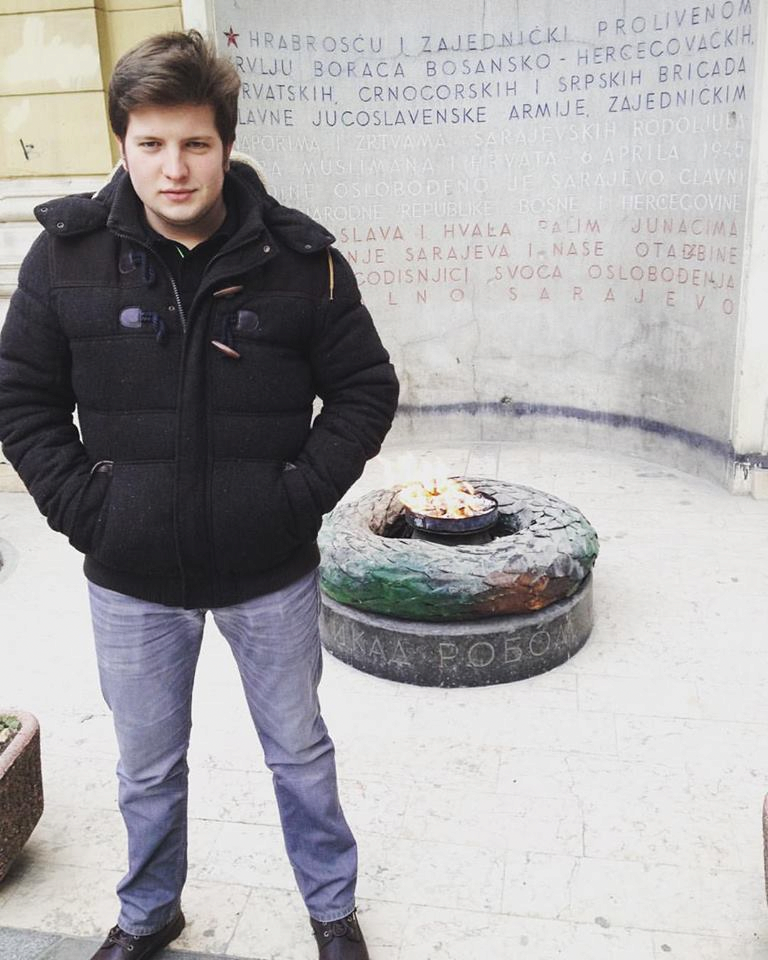
\includegraphics[scale=0.3]{../benchmark_results/pattern/3_components-1_bits.png} \\
3 & 2 &25\% & 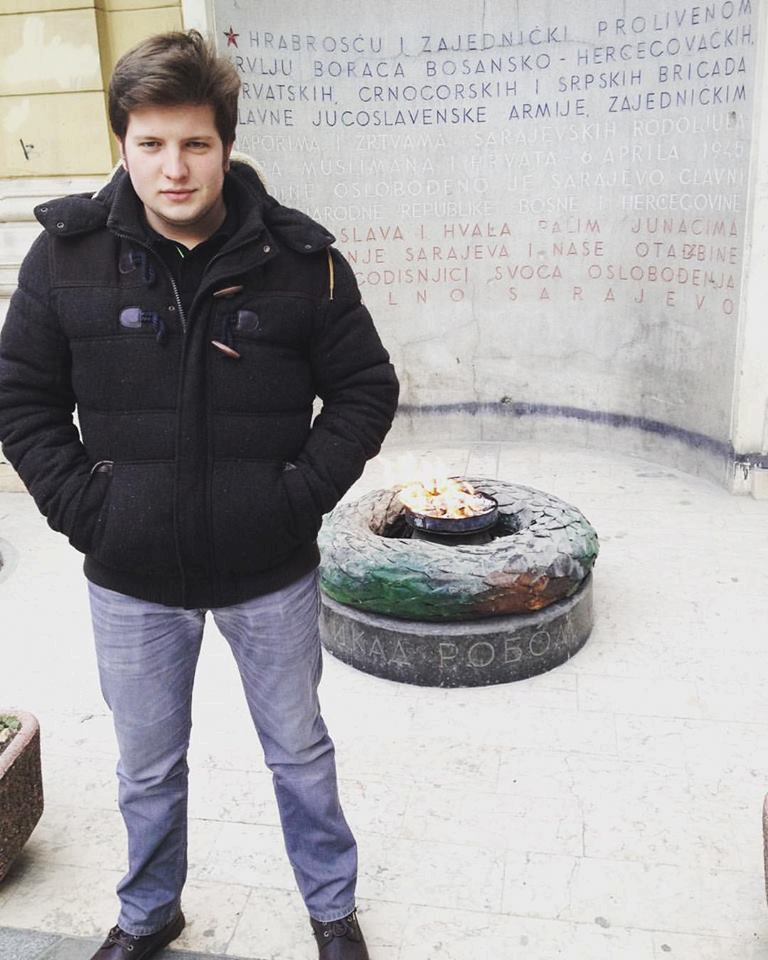
\includegraphics[scale=0.3]{../benchmark_results/pattern/3_components-2_bits.png} \\
3 & 3 &38\% & 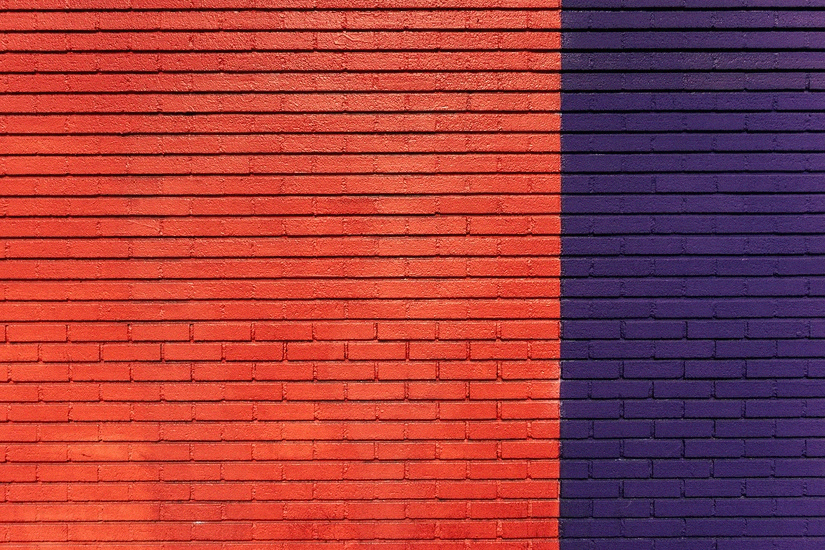
\includegraphics[scale=0.3]{../benchmark_results/pattern/3_components-3_bits.png} \\
3 & 4 &50\% & 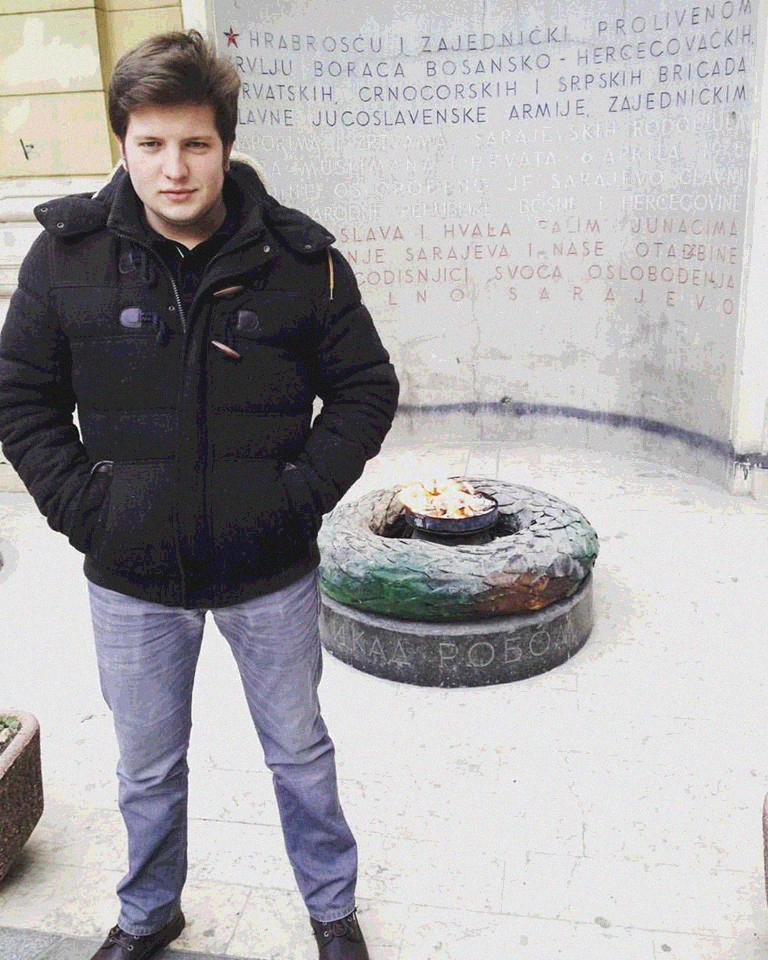
\includegraphics[scale=0.3]{../benchmark_results/pattern/3_components-4_bits.png} \\
3 & 5 &62\% & 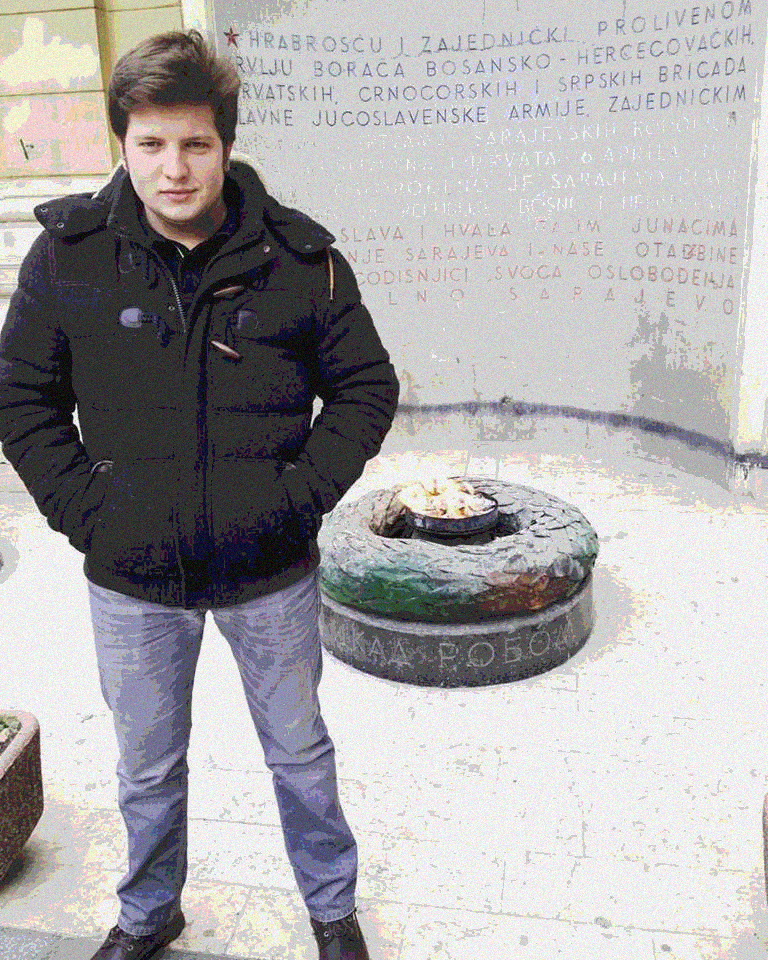
\includegraphics[scale=0.3]{../benchmark_results/pattern/3_components-5_bits.png} \\
3 & 6 &75\% & \includegraphics[scale=0.3]{../benchmark_results/pattern/3_components-6_bits.png} \\
3 & 7 &88\% & \includegraphics[scale=0.3]{../benchmark_results/pattern/3_components-7_bits.png} \\
3 & 8 &100\% & \includegraphics[scale=0.3]{../benchmark_results/pattern/3_components-8_bits.png} \\
\end{longtable}
\end{center}

\section{Analiza rezultata}
\paragraph{}
Ispitivanje je pokazalo kako upisana količina podataka znatno može utjecati na promjenu izgleda izvorne slike. Bez obzira na prirodu izvorne slike, za $\eta$ > 50\% obrađena slika sadrži znatnu količinu šuma, i nikako se ne preporučuje korištenje algoritma s parametrima $n_{bits}$ i $n_{componets}$ za $\eta$ > 50\%. Nadalje, parametri $n_{bits}$ i $n_{componets}$ za $\eta$ < 25\% generiraju slike za koje se ne može razlučiti da je nad njima vršena obrada. Iz ovog područja algoritam se najbolje ponaša za one parametre koji svaki kanal mijenaju u istoj mjeri iz razloga što je za te parametre izgled kontrasta na obrađenim slikama najprirodniji(svaka boja mijenja se u istj mjeri). Za $\eta \in$ [25\%, 50\%] algoritam daje prihvatljiva rješenja, ali samo za one parametre koji svaku komponentu boje mijenjaju u istoj mjeri. Za parametre iz tog intervala koji primjerice mijenjaju 7 bitova samo jedne komponente, slika poprima neprirodan izgled i u velikoj mjeri odskače od izgleda izvorne slike.
\paragraph{}
Analiza rezultata potvrđuje izvornu hipotezu da je algoritam osjetljiv na količinu podataka koji se upisuju na sliku. Najbolji rezultati ostvareni su za parametre koji mijenjaju do 2 najmanje značajna bita svake komponente(za $\eta \in$ [0\%, 25\%]), što u konačnici znači da se u svaku sliku može upisati količina podataka koja odgovara četvrtini veličine izvorne slike.
\chapter{Opis programske implementacije rješenja}

\chapter{Zaključak}

\bibliography{literatura}
\bibliographystyle{fer}

\end{document}
